% main.tex: the draft's source from C2p unit 2 on (STATE Blocked 108 (a)); edited by hand, never generated.
% Started as tex/main.tex (the conversion of draft-C2.md); `python -m trackC_writeup.paper_check` lists
% every number here that no record renders to. Upload this folder to Overleaf; it compiles with pdfLaTeX.
\documentclass[11pt]{article}
\usepackage[utf8]{inputenc}
\usepackage[T1]{fontenc}
\usepackage{lmodern}
\usepackage[margin=1in]{geometry}
\usepackage{amsmath,amssymb}
\usepackage{graphicx}
\usepackage{booktabs,tabularx}
\usepackage{caption}
\captionsetup[table]{position=top}
\usepackage[section]{placeins}
\usepackage[round,sort]{natbib}
\usepackage[hidelinks]{hyperref}

\title{Counting where a language model's token energy falls with depth: a break early in training, at falls of the tokens' mean}
\author{}
\date{}

\begin{document}
\maketitle

\begin{abstract}
We count, at 18 checkpoints of \texttt{pythia-410m} and of its nine PolyPythias seeds, on seven prompts, the layers at which the interaction energy $E_{1}$ of the unit-normalised tokens falls with depth. At $\beta $ = 1 the count's drops are falls of the tokens' mean: $E_{1}$'s first-order term is half the squared norm of the mean unit token, at every checkpoint the mean's norm falls at 0.96 or more of the transitions at which $E_{1}$ falls, and at the break every drop the count counts is a layer at which the mean's norm falls (how many of the mean's falls the count misses is not read). The count is zero through step 128 on seed 0 and reaches half its early plateau at step 512; a prediction registered before the seeds' intermediate checkpoints were downloaded put each seed's break at 256 or 512, and it held on 9 of 9, which shows the date is the training recipe's rather than one run's, and says nothing about mechanism. At the break the mean is spread over the model's coordinates as over a random basis, and the model's massive-activation coordinates are ordinary there. With each prompt's mean token removed, the count breaks one grid step later on seed 0, at 1000, and at 1000 on eight of the nine seeds. Editing every head's OV map does not undo the break: its symmetric part and its rotation removed leave the count as random edits of their size do, and its step-128 map lowers the count at steps 512 and 1000 beyond every random edit, to about half, but leaves it far from monotone. Every dated event falls inside the learning-rate warmup, and neither a different peak rate (\texttt{pythia-70m}, \texttt{pythia-160m}) nor a different warmup (Mistral's GPT-2 small) separates the dates from the schedule. The motivation is the particle picture of self-attention, in which, under identity weights, $E_\beta $ never decreases with depth. The results are exploratory except the registered seed count, on one model size, seven hand-picked prompts and a grid with no checkpoint between 512 and 1000.
\end{abstract}

\section{Introduction}\label{sec:1}

Read a transformer's depth as time and its tokens as particles on a sphere, and self-attention becomes an interaction between them \citep{geshkovski2023}. Under the simplest weights (one head with Q = K = V = I, the same in every layer) the particles attract and cluster, and the interaction energy $E_\beta $ of \S\ref{sec:2.1} never decreases with depth. That picture organises a growing theory of clustering and metastability (\S\ref{sec:8}). Trained language models do not follow it: at the end of its training, \texttt{pythia-410m}'s $E_{1}$ falls between consecutive layers 70 times over our seven prompts, out of 24 $\times $ 7 layer-to-layer transitions. No theorem is broken, since none covers a trained model (\S\ref{sec:2.1}), but the picture's prediction fails, and nothing says when along training it starts to fail, or what else is changing then.

We read $E_{1}$ layer by layer at 18 checkpoints of \texttt{pythia-410m} and of nine retrained seeds, counting V, the drops between consecutive layers (\S\ref{sec:3}). At $\beta $ = 1 the drops V counts are falls of the tokens' mean norm (\S\ref{sec:4.1}), so what V dates is, descriptively, the tokens' anisotropy ceasing to rise with depth; the particle picture is why we read it, not what it measures. We report two dated events, their place on the model's developmental order, and one negative result:

\begin{enumerate}
  \item \textbf{The break, dated and reproduced (\S\ref{sec:4}).} Through step 128 $E_{1}$ is monotone in depth on every prompt (V = 0 on seed 0); V reaches half its 1000--4000 level at step 512. A prediction registered before any seed's intermediate checkpoints were downloaded put the break at 256 or 512 on each of nine PolyPythias seeds, and it falls there on 9 of 9. The date is the recipe's, not one run's; with seeds that share the recipe this was the expected outcome, and the registration guards only against choosing the window after seeing them (\S\ref{sec:3.4}).
  \item \textbf{The token-centred cloud breaks later (\S\ref{sec:4.1}).} $E_{1}$'s first-order term is half the squared norm of the tokens' mean (\S\ref{sec:2.1}). With each prompt's mean token removed before normalising, the centred count at 512 on seed 0 is 0.19--0.24 of its own late level, where the uncentred count is at 0.98 of its own; the centred cloud's break comes at 1000, on seed 0 and on eight of the nine seeds at every tolerance read: one grid step after the break on the seeds that break at 512, two on those that break at 256. That is the step at which the previous-token and induction heads are dated, but by \S\ref{sec:5}'s convention the uncentred break, one grid step earlier, is as close to them, so the shared step is not read as a link. The two counts' sizes are not compared, only their dates. What the mean carries is read from $E_{1}$'s series instead, after the dates: at every checkpoint $E_{1}$ and $\|m\|^{2}$ change in the same direction at 0.956 or more of the transitions, and the mean's norm falls wherever V counts a drop at the break (at each of its 1224 drops from step 128 to 1000) and, at every step of training, at 0.96 or more of the layers at which $E_{1}$ falls by any amount. No privileged coordinates of the kinds we tested carry that mean at the break: the massive-activation coordinates are ordinary there and arrive at step 16 000 or later, and the mean and its falls are no more concentrated in the model's coordinates than in a random basis.
  \item \textbf{The timeline (\S\ref{sec:5}).} On seed 0 the break comes after the token cloud's rank collapse (step 8) and the unigram minimum (128); the bigram minimum (256), the fall in the OV maps' attractive share (512) and the previous-token and induction heads (1000) are each within one grid step of it, which we count as aligned, not ordered, since these are different kinds of quantity dated by different statistics (item 2's two counts are one statistic, \S\ref{sec:4.1}). \textbf{``Break, then induction, then the OV maps' repulsive phase'' is not shown:} in either reading of that phase it ties the break or induction on this grid.
  \item \textbf{One intervention, no reversal (\S\ref{sec:6}).} Making every head's OV map symmetric, or removing its rotation, does not take the break back towards monotone at any step after it; giving every head its own step-128 OV map lowers V at 512 and 1000 but leaves it far from monotone. The break is neither shown to be the OV maps' nor shown not to be.
\end{enumerate}

\textbf{What none of this separates (\S\ref{sec:7}).} Every dated event from step 128 to 1000 falls inside the learning-rate warmup, which runs to step 1430 and which all ten runs share. Two further runs do not separate a training event from the schedule. On \texttt{pythia-70m} and \texttt{pythia-160m}, which warm up over the same steps at higher peak rates, both dates are consistent with the count of updates and with the cumulative learning rate, and the centred date excludes the rate itself. On Mistral's GPT-2 small, whose warmup is logarithmic and longer, the break's larger rise falls where the count of updates predicts, after a smaller first rise where the cumulative rate does, and the label the rule fixed before that run gives turns on two of its choices (the plateau window and one tolerance of the centred count). So the dates are dates inside a warmup, not training events told apart from it. A released retraining of \texttt{pythia-70m} with a ten times longer warmup could tell them apart for that model, not for \texttt{pythia-410m}; it was found after these runs and is not read here (\S\ref{sec:7}).

Everything here is exploratory, on one model size, seven hand-picked prompts and a grid with no checkpoint between 512 and 1000; only the seed count of \S\ref{sec:4} was registered. \S\ref{sec:2} gives the energy and the exact conditions under which it is monotone, \S\ref{sec:3} the setup, \S\ref{sec:8} related work; appendix~\ref{sec:A} reads the heads' shared subspaces along the same steps, appendix~\ref{sec:B} the gate each reading passed before it was read, appendix~\ref{sec:C} what the count is made of (by prompt, by layer, without the frame-changing transitions, and $E_{1}$'s net change), and appendix~\ref{sec:D} takes the timeline's rows one by one: what each measures, why it is there, how it is dated and whether its change is larger than its noise.

\section{Background}\label{sec:2}

\subsection{The energy, and when it is monotone in depth}\label{sec:2.1}

Put each token's residual-stream state on the unit sphere, $x_{i} \in S^{d-1}$, i = 1, \dots{}, n, and let

\begin{equation}
E_\beta(X) = \frac{1}{2\beta n^2}\sum_{i}\sum_{j}\exp\bigl(\beta\,\langle x_i, x_j\rangle\bigr).
\end{equation}

$E_\beta $ is large when the tokens are close together and is maximised by a single cluster; over probability measures on the sphere its minimiser is the uniform one \citep[Prop. 3.4]{geshkovski2023}. Read a transformer's depth as continuous time for an interacting-particle system, with self-attention the interaction. When every layer has the same single head with Q = K = V = I, $E_\beta $ is non-decreasing in depth \citep[\S{}3.2]{geshkovski2023}, and the dynamics are a gradient ascent of $E_\beta $ in a metric that reweights the tokens \citep[\S{}3.4]{geshkovski2023}; with V = $-$I it is non-increasing. Wider hypotheses give monotonicity of a different, weighted energy, not of $E_\beta $: for one head whose score matrix $Q^{\top}$K is symmetric and equal to V, the dynamics ascend (1/2$\beta $) $\sum _{ij}$ exp($\beta \langle Vx_{i}, x_{j}\rangle $) in a metric that weights each token by its attention normaliser \citep[\S{}3.4.1]{geshkovski2023}, and for many heads whose score matrices are each symmetric and equal (or close) to their value maps, a sum of energies weighted by those matrices is non-decreasing \citep[Theorems 11--12]{pendharkar2026}, though a single head's own energy on the sphere is monotone only under a further condition, because cross-head radial terms enter its derivative \citep[\S{}4.2, Theorem 17]{pendharkar2026}. No monotonicity result for $E_\beta $ covers MLP blocks, values untied from the scores, weights that change from layer to layer, or discrete layers. Tying the values to the scores is that theory's main idealisation \citep[Remark 5]{pendharkar2026}; in a trained transformer they are separate parameters. The nearest result to an initialised model is about one term of $E_\beta $, not $E_\beta $ itself: for attention-only layers whose weights are drawn independently across layers and heads, as at initialisation, at a small attention inverse temperature, and from tokens whose pairwise overlaps all start positive, the tokens' mean overlap, $\|m\|^{2}$ below, follows a logistic curve that rises with depth, with high probability \citep{koubbi2026}. Our step-0 inputs do not meet the last condition (about half of each prompt's pairs of step-0 token embeddings have a negative cosine), so that result is context here, not a prediction.

So no theorem says a trained language model's $E_\beta $ should be monotone in depth, and none says a randomly initialised one's should. We read monotonicity as the prediction of the identity-weight picture, and a drop in $E_\beta $ between consecutive layers as a departure from that picture, not as the violation of a theorem. That this model at initialisation is monotone or nearly so (seed 0 has no drop at step 0, five of the nine further seeds a few; \S\ref{sec:4}), and a trained one is not, is then an empirical fact about this model, which \S\ref{sec:4} dates.

$E_\beta $ sums over all pairs of tokens, so its first-order term is set by the tokens' mean. With m = (1/n) $\sum _{i} x_{i}$, expanding the exponential gives, exactly,

\begin{equation}
E_1 = \tfrac12 + \tfrac12\,\|m\|^2 + \sum_{k\ge 2}\frac{1}{2n^2\,k!}\sum_i\sum_j \langle x_i, x_j\rangle^k,
\end{equation}

where $\|m\|^{2}$, the squared norm of the mean, is a standard measure of anisotropy (\S\ref{sec:8}): for unit tokens the mean cosine between distinct tokens, the measure of \citet{ethayarajh2019} applied to one prompt, is exactly $(n\|m\|^{2}-1)/(n-1)$. The higher terms are not small (|$\langle x_{i}, x_{j}\rangle $| $\leq $ 1, and the n diagonal terms are 1) and none is negative, since $\sum_i\sum_j\langle x_i, x_j\rangle^k = \|\sum_i x_i^{\otimes k}\|^2$; so $E_{1}$ is not $\|m\|^{2}$, but a drop in $E_{1}$ between layers can come from the mean shrinking alone. \S\ref{sec:4.1} removes the mean.

\subsection{The developmental order}\label{sec:2.2}

Language models acquire their internal structure in stages. In a small two-layer attention-only model, \citet{hoogland2024} find bigram statistics first, then positional use and common 3- and 4-grams, then previous-token heads, then induction heads, then a long stage with no significant change, each stage a period of change in the local learning coefficient; that model was trained at a constant learning rate, so there the order is not a warmup's. Induction heads form at the point where in-context learning improves abruptly, visible as a bump in the training loss \citep{olsson2022}. On Pythia, a model's loss on sequences sampled from unigram and bigram statistics falls to a trough between steps $2^{6}$ and $2^{8}$ and rises until about $2^{10}$ \citep{belrose2024}, and task-level components emerge at similar token counts across model sizes, induction heads soon after $2 \times 10^{9}$ tokens \citep{tigges2024}, about step 950 at Pythia's tokens per step. \S\ref{sec:5} places the energy's break on this order for one model, \texttt{pythia-410m}, with every row dated by the same locator.

\subsection{Pythia's training, and its warmup}\label{sec:2.3}

The Pythia models are trained for 143 000 steps of 1024 sequences of 2048 tokens \citep{biderman2023}, with the learning rate warmed up linearly over the first 1 \% of training (1430 steps) and decayed by a cosine to 0.1 of its peak; the peak is 3 $\times 10^{-4}$ for \texttt{pythia-410m}, 6 $\times 10^{-4}$ for \texttt{pythia-160m} and $10^{-3}$ for \texttt{pythia-70m} \citep{biderman2023}, and the released training configs warm the two smaller models up over the same 1430 steps. The suite releases checkpoints at steps 0, 1, 2, 4, 8, 16, 32, 64, 128, 256, 512 and then every 1000 steps. Every early event \S\ref{sec:4} and \S\ref{sec:5} date, the energy's break included, therefore falls inside the warmup, and nothing in one schedule separates a change caused by training from one caused by the schedule. \citet{li2025} tie the first of their three geometric phases to the same ramp. PolyPythias \citep{vanderwal2025} retrains \texttt{pythia-410m} from nine further seeds with the same schedule, which lets \S\ref{sec:4} ask whether the break's step is the run's or the recipe's, but not whether it is the schedule's (\S\ref{sec:7}).

\section{Setup}\label{sec:3}

\subsection{The model, the checkpoints and the prompts}\label{sec:3.1}

\texttt{pythia-410m} has 24 layers of width 1024, each with 16 attention heads (384 in all); each block adds its attention and its MLP to the residual stream in parallel, and positions enter through rotary embeddings \citep{biderman2023}. We read 18 of its checkpoints, steps 0, 2, 4, 8, 16, 32, 64, 128, 256, 512, 1000, 2000, 4000, 8000, 16 000, 32 000, 54 000, 143 000 (the set earlier readings of this model used, which is why it holds 54 000 rather than 64 000). Step 1 is left out: in our runs its outputs are identical to step 0's (we did not compare the weights), so it adds no point. There is no checkpoint between 512 and 1000, or between 1000 and 2000, so nothing below dates a change more finely than the grid.

PolyPythias \citep{vanderwal2025} retrains \texttt{pythia-410m} from nine further random seeds, \texttt{pythia-410m-seed1} to \texttt{pythia-410m-seed9}, with the same code, data and schedule but a different initialisation and batch composition (how documents are packed into sequences), and releases the same checkpoints; we call the original run seed 0. PolyPythias reports two of the nine, seeds 3 and 4, as outlier runs; we keep both and flag them, as fixed before any of their checkpoints was read.

Every seed and step reads the same seven texts: a passage of Camus's \emph{L'Étranger} in French, a method from the Python source of the HDBSCAN library, a passage of the \emph{Iliad} in English translation, the source of a LaTeX document, a paragraph from a paper on transformers, Sullivan Ballou's 1861 letter to his wife, and a Wikipedia paragraph on Charlotte Brontë, each cut at 512 tokens (prompt-set hash \texttt{976b62d677bc}). They span two languages, prose, verse, code and markup, but they are few and were chosen by hand, not sampled, and every count below is a count over these seven. Forward passes run in float32 with TF32 off, on one GPU. On seed 0 the per-state energies reproduce an earlier CPU run of this project to a relative 1.5 $\times 10^{-6}$, and the counts of \S\ref{sec:3.2} exactly.

\subsection{The energy and the drop count}\label{sec:3.2}

At each checkpoint and prompt we take the residual stream's 25 states as the model returns them: the token embeddings, the outputs of the first 23 blocks, and the last block's output after the final layer norm. Each token's vector is normalised to unit length, so a prompt's n tokens lie on the sphere, and $E_{1}$ of \S\ref{sec:2.1} ($\beta $ = 1) is computed at each state, every position included. A step from one state to the next is a \emph{drop} when $E_{1}$ falls by more than a fraction $10^{-3}$ of its value. \textbf{V}, the statistic of everything below, is the number of drops at one checkpoint: over the 24 transitions of each prompt, summed over the 7 prompts, so at most 24 $\times $ 7. Two of the transitions change frame as well as layer (the embeddings into the first block's output, and the last block's output into the final layer norm); they are counted like the rest, they hold none of the drops from step 256 to 1000 on any seed, and V counted without them dates every seed's break at the same step (appendix~\ref{sec:C}). V is not one prompt's: at each seed's break no prompt holds more than 0.24 of it (an even split is 0.14). And a drop is a dip, not a net fall: on every prompt, seed and step, $E_{1}$ is higher after the last state than at the embeddings (appendix~\ref{sec:C}, with figure~\ref{fig:fig5_count}'s map of where the drops sit). In the identity-weight picture V is 0. A drop is a departure from that picture's prediction, not the violation of a theorem (\S\ref{sec:2.1}). The tolerance keeps float noise out of the count; on seed 0 the break's date below is 512 at each of the tolerances $10^{-4}, 10^{-3}$ and $10^{-2}$, and 512 with any one prompt left out.

$\beta $ = 1 is the one setting seed 0 had been read at before the seeds were registered (\S\ref{sec:3.4}); no other $\beta $ is read in this frame. A second energy, $E_{3.5}$ in each block's input frame (after its first layer norm, positions 1 to n $-$ 1, blocks 0 to 23), is read beside it in \S\ref{sec:4} and never counted; $\beta $ = 3.5 is a value we fitted earlier to this model's attention scores, and the frame is the one attention reads.

\subsection{Dating the break}\label{sec:3.3}

Let m be the median of V over steps 1000, 2000 and 4000. The break's step is the first grid step at which V $\geq $ m / 2, a \emph{half-rise}. The plateau is early on purpose: V keeps moving late in training (on seed 0, 57 on the plateau and 70 at the last step), and a reference taken there would let a late rise move an early date. Read after the dates with the plateau at 8000--32 000 instead (median 59--74 drops by seed), every seed's half-rise stays in (128, 512] and only seed 9 moves, from 256 to 512 (appendix~\ref{sec:C}). Two other rules were set aside on seed 0 before the seeds were read: the first step with V > 0 moves with a single stray drop, and V's change-weighted centroid in log step lands at about 827 on seed 0, pulled late by the rise between 16 000 and 32 000.

\subsection{What was registered, and when}\label{sec:3.4}

Before any seed's checkpoints between its first and last were downloaded, we committed a prediction, \texttt{P-A5}, to this project's registry of predictions, kept in its git history: on each of the nine seeds the break falls at 256 or 512, a window (128, 512] chosen after seed 0 was read, with seed 0's step at its right edge. K counts the seeds inside. The registered falsifier was K $\leq $ 3, so under the null below the prediction escapes its falsifier (K $\geq $ 3 + 1) with probability 0.048. The null puts each seed's step uniformly and independently on the 12 non-zero grid steps up to 4000, so under it K \textasciitilde{} Bin(9, 1/6); p = P(Bin(9, 1/6) $\geq $ K), exact, and the e-value is E = $\kappa p^{\kappa -1}$ with $\kappa $ = 0.5, a p-to-e calibrator fixed before the run \citep{vovk2019}. Nobody holds that null. It says the step is the run's, scattered over the early grid; it is the alternative to ``the step is the recipe's'', and beating it says only that. PolyPythias already reports training dynamics highly consistent across seeds, and every seed shares the recipe, so 9 of 9 was the expected outcome; what the registration adds is that the window was fixed before any seed's intermediate checkpoint was seen.

The registration commit (\texttt{c2eb9a7}) is dated 2026-10-20, 18:36 UTC; the first seed record was written at 18:39 UTC the same day, 3 minutes later. Both times are written by us: a commit's date is set by its author, and the record's time by our code. The earliest time outside our control is GitHub's activity log, which records the creation of the branch carrying the registration commit at 18:38 UTC, before the first seed record's 18:39; the log keeps such events for about 90 days, so a copy is kept with the code. Every seed's first and last checkpoints were already on disk, and earlier work of ours had read the first.

\subsection{Notation and terms}\label{sec:3.5}

\begin{description}
  \item[$x_{i}$, n, m, $\|m\|^{2}$.] A token's residual-stream state normalised to unit length; the prompt's number of tokens; their mean, m = (1/n) $\sum _{i} x_{i}$; its squared norm, the anisotropy measure of \S\ref{sec:2.1}.
  \item[$E_\beta $, $E_{1}$.] The interaction energy of \S\ref{sec:2.1}; $E_{1}$ is it at $\beta $ = 1, the only $\beta $ counted.
  \item[Drop, V, $V_c$.] A drop is a transition between consecutive states at which $E_{1}$ falls by more than the tolerance; V is the number of drops at one checkpoint over the 7 prompts (\S\ref{sec:3.2}); $V_c$ is the same count on the token-centred cloud (\S\ref{sec:4.1}).
  \item[Plateau, half-rise, break.] The plateau is V's median over steps 1000, 2000 and 4000; the half-rise is the first grid step at which V reaches half of it; the break is V's half-rise, and the centred date $V_c$'s (\S\ref{sec:3.3}).
  \item[Grid step.] One of the 18 checkpoints read; ``within one grid step'' means equal or adjacent on that list.
  \item[Seed 0, the nine seeds, K.] Seed 0 is the original \texttt{pythia-410m} run, the nine seeds are PolyPythias' seeds 1--9, and K is the number of the nine whose break falls in the registered window (128, 512] (\S\ref{sec:3.4}).
  \item[Fixed before the run.] A rule written down and committed before any of its outputs was computed.
  \item[Gate.] A run of a reading's full statistic, before the real data are read, on inputs whose answer is known: a planted null and a planted effect at the real design points (appendix~\ref{sec:B}). A gate that fails \emph{refuses} the reading until the rule is changed, and the change is stated.
  \item[Arm.] One variant of a reading run beside the others under the same rule, for example one tolerance of the centred count, or one projection of \S\ref{sec:4.1}.
  \item[Description.] A reading with no calibrated null, or one read after the dates it might have moved; it is reported, not tested, and no date rests on it.
  \item[Locator.] \S\ref{sec:5}'s rule for dating a row of the timeline; each row is defined and read in appendix~\ref{sec:D}.
\end{description}

\section{The break, dated and reproduced}\label{sec:4}

\begin{figure}[tbp]
\centering
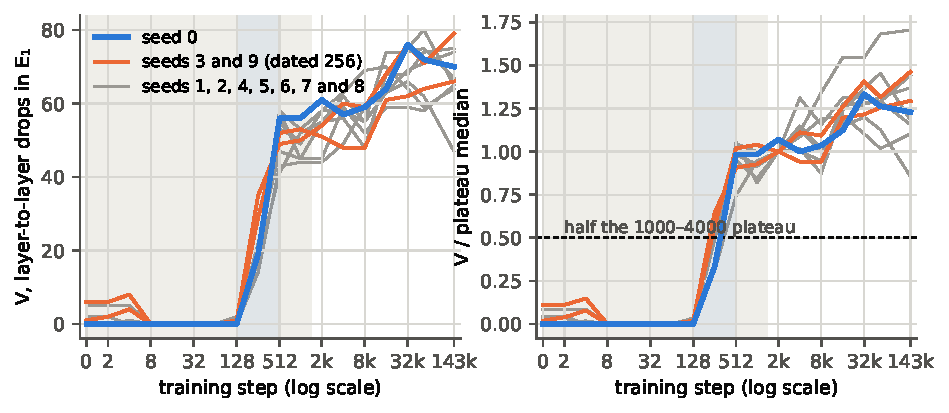
\includegraphics[width=\linewidth]{fig/fig1_break.pdf}
\caption{V, the number of layer-to-layer drops in $E_{1}$ over the 7 prompts, at each of the 18 steps, for seed 0 (blue) and the nine PolyPythias seeds; seeds 3 and 9, dated 256, in orange; the other seven in grey, not told apart (seed 4, the other outlier run, among them). Left, V; right, V over each run's 1000--4000 plateau median, with the half-rise line. Light blue band: the registered window (128, 512]. Grey shading: the learning-rate warmup, to step 1430. Step 0 is drawn one octave left of step 2, where step 1 would be.}\label{fig:fig1_break}
\end{figure}

\textbf{Seed 0.} V is 0 at every step up to 128: on no prompt does $E_{1}$ fall by more than the tolerance from one of its 25 states to the next. It is 19 at 256 and 56 at 512, against a plateau median of 57, so the half-rise dates the break at \textbf{512} (figure~\ref{fig:fig1_break}), and V stays high to the end of training (70 at the last step).

\begin{table}[tbp]
\centering\small
\caption{V on each run at the steps around the break, its 1000--4000 plateau median, and the break (V's half-rise, \S\ref{sec:3.3}). Seed 0 is the original run; seeds 1--9 are PolyPythias', 3 and 4 its outlier runs. The registered window is (128, 512].}\label{tab:seeds}
\begin{tabular}{@{}rrrrrrrr@{}}
\toprule
seed & V at 0 & 128 & 256 & 512 & 1000 & plateau & break \\
\midrule
0 & 0 & 0 & 19 & 56 & 56 & 57 & 512 \\
1 & 2 & 0 & 22 & 47 & 45 & 45 & 512 \\
2 & 0 & 1 & 17 & 41 & 52 & 55 & 512 \\
3 & 6 & 1 & 35 & 49 & 50 & 54 & 256 \\
4 & 0 & 1 & 18 & 58 & 45 & 55 & 512 \\
5 & 2 & 2 & 18 & 55 & 49 & 58 & 512 \\
6 & 0 & 0 & 17 & 53 & 50 & 54 & 512 \\
7 & 0 & 0 & 14 & 43 & 44 & 44 & 512 \\
8 & 5 & 1 & 19 & 58 & 53 & 58 & 512 \\
9 & 1 & 1 & 29 & 52 & 53 & 51 & 256 \\
\bottomrule
\end{tabular}
\end{table}

\textbf{The nine seeds} (table~\ref{tab:seeds}). The break falls inside the window on all nine: \textbf{K = 9 of 9}. Seven seeds date it at 512, as seed 0 does; seeds 3 and 9 date it at 256. Both outlier runs, seeds 3 and 4, are inside. No seed is near the window's edges: at 128 every seed's V is at most 2, against half-plateau lines of at least 22; at 512 every V is at least 41, against lines of at most 29. A count that moved by one drop could move a seed between 256 and 512, never out of the window. Against the registered null of \S\ref{sec:3.4}, which nobody holds, K = 9 gives p = 9.9 $\times 10^{-8}$ and E = 1587; we report them because they were registered, not as the strength of the result.

\textbf{What K = 9 says, and what it does not.} The break's step belongs to 410m's recipe, not to one run: the date \S\ref{sec:5} places on the developmental order is the recipe's. It does not separate a training event from the learning-rate schedule. Every seed shares the warmup, which runs to step 1430, past the whole window, so a break set by the schedule's ramp would reproduce exactly as this one does (\S\ref{sec:7}). And the null it beats is one nobody holds, so a large E here is cheap: the check makes the date reproducible, and is evidence neither about mechanism nor that trained weights resist the clustering the particle picture describes.

\textbf{Beside the count} (fixed before the run, never scored):

\begin{itemize}
  \item \emph{Step 0 is not monotone on every seed.} Seeds 1, 3, 5, 8 and 9 show 1--6 drops at step 0 (seed 0 none), up to 8 at step 4 (seed 3); V is 0 at steps 8 to 64 on every seed. Against plateaus of 44--58 these are small, but ``monotone at initialisation'' holds for seed 0 and four of the nine seeds, not for all ten. That the early drops are gone by step 8, the step the token cloud's rank collapse is dated (\S\ref{sec:5}), is seen, not read further.
  \item \emph{The second energy dates the break inside the window too.} $E_{3.5}$ in each block's input frame dates it at 512 on 9 of the 9 seeds, and at 512 on seed 0, so it differs from $E_{1}$'s date on seeds 3 and 9, which $E_{1}$ dates at 256.
\end{itemize}

\subsection{The token-centred cloud}\label{sec:4.1}

$E_{1}$'s first-order term is $\tfrac12\|m\|^{2}$, the squared norm of the tokens' mean (\S\ref{sec:2.1}), so a direction all tokens share, growing or shrinking from layer to layer, moves $E_{1}$ with no change in how the tokens sit relative to one another (\S\ref{sec:8}). To remove it, at each state we take the unit token cloud, subtract the prompt's mean unit token and normalise each row again, and count the drops in $E_{1}$ of this centred cloud, $V_c$, with the same half-rise. (Normalising after centring leaves a small mean, so the centred cloud is not exactly mean-free.) The rule was fixed before any centred number was read. Centring changes $E_{1}$'s scale, so $V_c$ is counted at four tolerances: $10^{-4}$ and 3 $\times 10^{-4}$, fixed, and 7.6 $\times 10^{-5}$ and 7.6 $\times 10^{-4}$, derived from the uncentred count's behaviour, the first so that the same architecture at random initialisation drops as often centred as uncentred, the second so that a planted spread of the tokens is seen alike by both counts (appendix~\ref{sec:B}). A centred date counts only if it holds at all four. No single tolerance reads a planted change alike through both counts, so we compare their dates, never their sizes.

\textbf{Seed 0.} $V_c$ is at most 3 at every step through 128 across the four tolerances. At 512, where V is 0.98 of its plateau, $V_c$ is 0.19--0.24 of its own (5--11 drops); its half-rise is at \textbf{1000} at each tolerance. \textbf{The nine seeds.} The centred half-rise falls after the seed's uncentred break on eight of nine seeds, and at 1000 on eight; seed 6 has no centred date by that rule: three of its four tolerances date it at 1000 and one (3 $\times 10^{-4}$) at 512, its own break. Read after the dates: at the uncentred break $V_c$ is 0.07--0.50 of its own plateau on the seeds that break at 512 and 0.00--0.04 on the two that break at 256, below half on every seed but the one tie.

So, by the half-rise, the break at its step is not seen once the mean token is removed: the centred cloud has not yet broken at 256 or 512, and it breaks at 1000, the step where \S\ref{sec:5} dates the previous-token and induction heads (by \S\ref{sec:5}'s convention the uncentred break, one grid step earlier, is as close to them, so the shared step is not read as a link). This is a statement about dates. What the uncentred count is made of is read below: at $\beta $ = 1 every drop it counts at the break is a fall of the mean's norm, so the break at 512 is, descriptively, the tokens' anisotropy ceasing to rise with depth at some layers; what drives it is not read. The two counts are one statistic on the same states, dated by one rule fixed before the run, which reads a later grid step as later; \S\ref{sec:5}'s convention, under which a one-step gap between rows of different kinds counts as aligned, is not applied to them.

\begin{figure}[tbp]
\centering
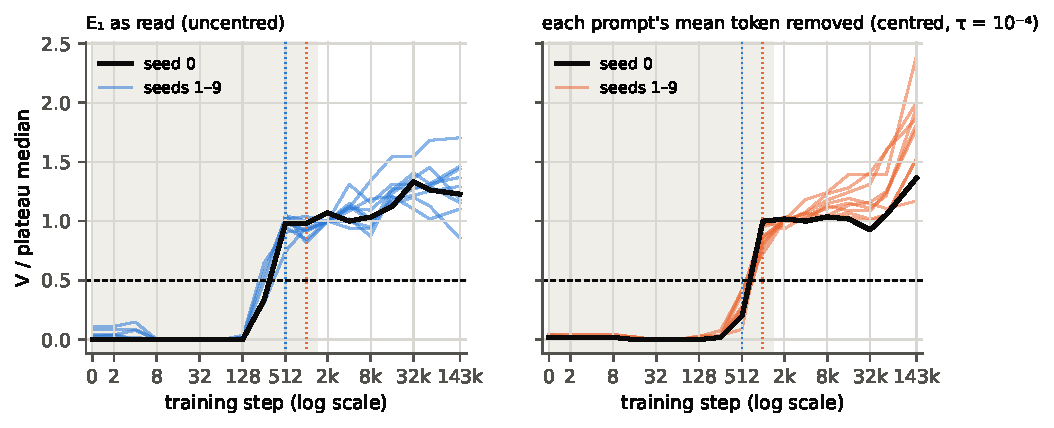
\includegraphics[width=\linewidth]{fig/fig7_events.pdf}
\caption{The two events on the ten seeds. Left, V over each seed's plateau median (figure~\ref{fig:fig1_break}'s right panel); right, the centred count $V_c$ at tolerance $10^{-4}$ over its own plateau median. Dotted: steps 512 and 1000; dashed: half the plateau. By the four-tolerance rule the centred count's half-rise is at 1000 on eight of the nine seeds. Dates only: the two panels' heights are not comparable.}\label{fig:fig7_events}
\end{figure}

\emph{The mean's term by layer} (read after the dates; description). Averaged over the prompts, $\|m\|^{2}$ never falls from one state to the next at step 128 on any of the ten seeds; at 512 it falls at 6--10 of its 24 transitions on every seed, and at 256 the two seeds whose break is at 256 have the most falls. At steps 128 to 1000 the two frame-changing transitions hold none of the falls (later in training they do). So $E_{1}$'s first-order term stops rising with depth at the break, on every seed. That is the same break seen through one term of $E_{1}$, not separate evidence.

\emph{How much of V the mean's term carries} (read after the dates; description). Since $E_{1} = \tfrac12 + \tfrac12\|m\|^{2}$ + R exactly, with R $\geq $ 0 the sum of the higher terms (\S\ref{sec:2.1}; each is a squared norm), every change splits as $\Delta E_{1} = \tfrac12\Delta \|m\|^{2} + \Delta $R. The two terms move together almost always, and not only at the break: at every checkpoint, on the ten seeds and seven prompts, $E_{1}$ and $\|m\|^{2}$ change in the same direction at 0.956--1.000 of the transitions, and whenever $E_{1}$ falls by any amount $\|m\|^{2}$ falls at 0.96--1.00 of them. So at $\beta $ = 1 nearly every fall of $E_{1}$, at every step of training, is a layer at which the tokens' mean norm falls (how many of the mean's falls V does not count is not read); the drops at the break are no exception ($\|m\|^{2}$ falls at each of the 1224 drops from step 128 to 1000, and its term is more than half the drop at all but one, the median share 0.81--1.02 by step; a share above 1 means R rose while the mean's term fell). The mean's term is not always most of $E_{1}$'s change: on the rises at steps 16 and 32 it is more than half at only 0.30 and 0.43 of them (from step 128 on, at most rises). The split is exact but it does not separate the mean from the rest: when the tokens share a direction every $\langle x_{i},x_{j}\rangle $ is large, so R's higher terms carry the mean too, and R is not a mean-free energy (the centred cloud nearly is, up to the small mean that re-normalising leaves). (Comparing these against R's own count of drops would need a tolerance on R's scale, which shrinks along training, and none is calibrated; it is not read.)

\begin{figure}[tbp]
\centering
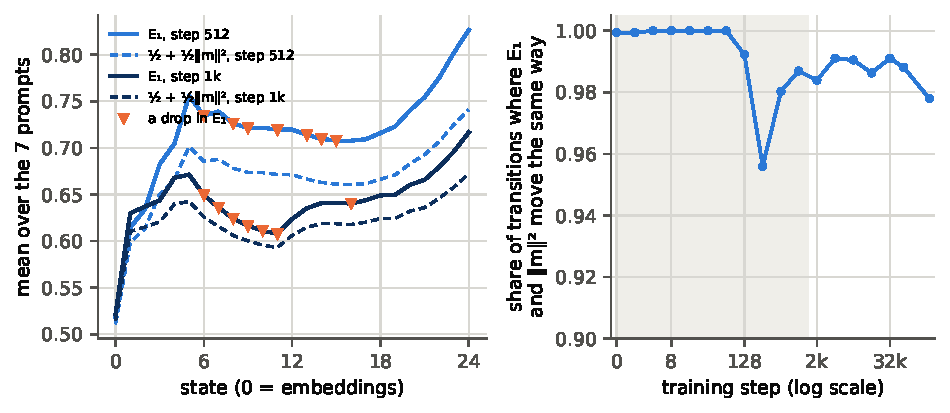
\includegraphics[width=\linewidth]{fig/fig8_mean.pdf}
\caption{Left, seed 0's $E_{1}$ by state at steps 512 and 1000 (solid) and its first two terms, $\tfrac12 + \tfrac12\|m\|^{2}$ (dashed), each averaged over the 7 prompts; the gap between a pair is the average of R $\geq $ 0. Triangles mark the transitions at which the averaged $E_{1}$ falls (not V's per-prompt drops). Right, the share of layer-to-layer transitions (ten seeds, 7 prompts, 24 transitions) at which $E_{1}$ and $\|m\|^{2}$ change in the same direction, by step.}\label{fig:fig8_mean}
\end{figure}

\emph{Which coordinates carry the mean} (read after the dates; description; a read-out of the states, not an intervention). Large language models carry a few coordinates of very large magnitude \citep{sun2024}, and a mean held by a few of them would make the break a property of the basis. At the break it is not. Half of $\|m\|^{2}$ takes 132--135 of the 1024 coordinates at 512 and 1000, against 127--129 for the same means in random bases (figure~\ref{fig:fig10_level}): the mean is spread over the model's coordinates as over a random basis. The falls V counts read the same way. By the rule fixed before the run, each of the 1224 drops from step 128 to 1000 asks whether the fall of $\|m\|^{2}$ is more concentrated in the model's coordinates than in 100 random rotations of it, and the falls are not basis-aligned on 9 of the 9 PolyPythias seeds (seed 0, read first to fix the rule, is not in this tally or in the projection's below; the other counts in this paragraph are over all ten); no coordinate is among a fall's carriers at a quarter or more of any seed's falls. The massive-activation coordinates, 2--3 per seed (those that reach 100$\times $ the median coordinate's largest value at some grid step: one set per seed, the union over the grid, not the set at the last step, which differs on some seeds), are ordinary at 128--1000, at most 2.35$\times $ (figure~\ref{fig:fig9_massive}), reach 100$\times $ at 16 000--32 000, and hold more than half of none of the 1224 falls. Projected out of every token, they leave the break's date where it was on 7 of the 9 seeds (on the other two one arm crosses the half line by one drop, as random coordinate sets of the same size also do) and the centred date on 9 of 9, each tolerance against its own unprojected date (so seed 6, which has no single centred date, counts as kept); since they are ordinary at these steps, that is a check rather than a test that could have moved. So, at the break, neither the massive set nor a concentration of the size the reading was gated on (3 coordinates holding most of each fall, a plant it detects) carries the falls. This is a statement about the basis, not a count: a few coordinates hold half of a \emph{net} fall in any basis, through cancellation among the rest, so it does not say the falls are spread over many coordinates. After the break the mean concentrates: half of $\|m\|^{2}$ takes 126--131 coordinates at 2000, fewer than a random basis on every seed at 4000 (104--113), and 2--3 at 16 000, as the massive coordinates arrive (appendix~\ref{sec:C}).

\begin{figure}[tbp]
\centering
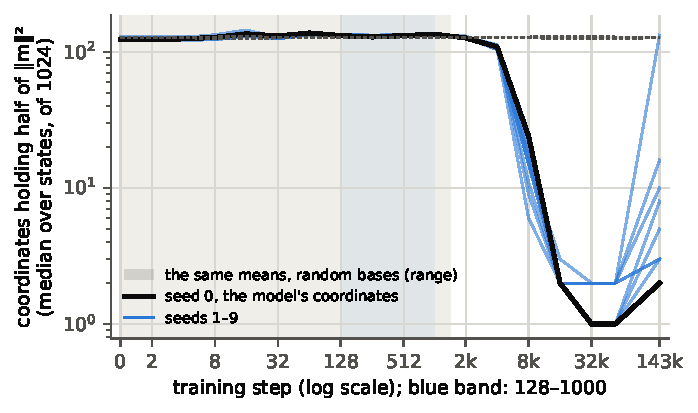
\includegraphics[width=\linewidth]{fig/fig10_level.pdf}
\caption{How many of the 1024 coordinates hold half of $\|m\|^{2}$ (median over the 25 states), by step: each seed in the model's own coordinates, and in grey the range over the seeds of the same means in random bases (dotted: its edges). At 512 and 1000 the two differ by a few coordinates, 132--135 against 127--129, too little to see on this scale.}\label{fig:fig10_level}
\end{figure}

The rule fixed for seed 0 before its run carried a size label, ``mostly removed'' (centred plateau 20 against 57, at that rule's tolerance $10^{-3}$), and we withdraw it: at the matched tolerance $10^{-4}$ the centred plateau is 0.96 of the uncentred one, so the label measured centring's change of scale, not a smaller break. That ratio is quoted only to withdraw the label; it is not a size reading.

\section{The timeline}\label{sec:5}

Where does the break fall against what else the model learns? On seed 0's 18 steps we dated the break among eight other changes measured on the model, the learning-rate schedule and a simulator's row, with one locator (table~\ref{tab:rows}, figure~\ref{fig:fig2_timeline}).

\textbf{The locator.} For a row x(s), signed so that its change is positive, let $\Delta $(s) = x(s) $-$ x(0). The reference is the largest $\Delta $ over steps up to 4000, and the row's step is the first at which $\Delta $ reaches half the reference. A row whose reference is under 4 bootstrap standard errors (over the row's prompts, heads, layers or text blocks) reads ``no change''. The two n-gram rows fall and then rise, and are dated at their minimum. The energy row E1 is dated by \S\ref{sec:3.3}'s half-rise instead, and the learning-rate row E10 by the same half-point with no floor. Before any real row was dated, the locator was gated on null series and on changes planted in each gap of the grid; the first gate failed on four rows, whose spread grows by orders of magnitude over training, and the revised gate passes on every row dated here (appendix~\ref{sec:B}). The locator dates a row's first move only; a row that later reverses is described, not dated again.

\begin{table}[tbp]
\centering\small
\caption{Seed 0's rows, ordered by their dated step; each row is taken on its own in appendix~\ref{sec:D} (a row's name links to its entry). All are on \texttt{pythia-410m}'s 18 steps and the 7 prompts, except the n-gram rows, read on 64 held-out text blocks from the Pile's validation split. E1c, the centred cloud (\S\ref{sec:4.1}), is dated by \S\ref{sec:3.3}'s half-rise and was added after the other rows were read. Censored: the row's largest change up to 4000 is at 4000, still growing, so its date is a lower bound. Refused: E11 runs the identity-weight dynamics from each step's measured token cloud and reads one cluster in every cell, as theory requires at a long horizon, so it cannot date anything. E3's two heads, and E4's, were named in earlier work on this model, not chosen by the seeds' rule of the 1000 tie below.}\label{tab:rows}
\begin{tabularx}{\linewidth}{@{}l X l@{}}
\toprule
row & what changes & dated step \\
\midrule
\hyperref[sec:D:E5]{E5} & effective rank of the token cloud on the sphere, mean over prompts, falls & 8 \\
\hyperref[sec:D:E6]{E6u} & KL divergence from a unigram predictor to the model's next-token distribution, at its minimum & 128 \\
\hyperref[sec:D:E6]{E6b} & the same for a bigram predictor (also 256 with the bigram counted on the rest of the split) & 256 \\
\hyperref[sec:D:E1]{E1} & the energy break (\S\ref{sec:4}) & 512 \\
\hyperref[sec:D:E2]{E2} & the OV maps' attractive share: per head, the share of the OV map's squared eigenvalue mass on eigenvalues with positive real part, median over the 384 heads, falls & 512 \\
\hyperref[sec:D:E8]{E8} & the weights' spectral tail exponent $\alpha $ \citep{martin2019}, median over matrix types and layers, falls & 1000 (512 from its peak) \\
\hyperref[sec:D:E3]{E3} & induction: attention of two induction heads (\texttt{L8H6}, \texttt{L11H14}) to the token after an earlier copy of the current one & 1000 \\
\hyperref[sec:D:E4]{E4} & previous-token attention of head \texttt{L5H2} & 1000 \\
\hyperref[sec:D:E1c]{E1c} & the token-centred cloud's break (\S\ref{sec:4.1}), the same at each of its four tolerances & 1000 \\
\hyperref[sec:D:E10]{E10} & the learning-rate schedule, its half-point & 1000 \\
\hyperref[sec:D:E7]{E7} & relative weight change $\|W - W_{0}\| / \|W_{0}\|$ & censored at 2000 \\
\hyperref[sec:D:E11]{E11} & a simulator's cluster count from the measured start & refused \\
\bottomrule
\end{tabularx}
\end{table}

\begin{figure}[tbp]
\centering
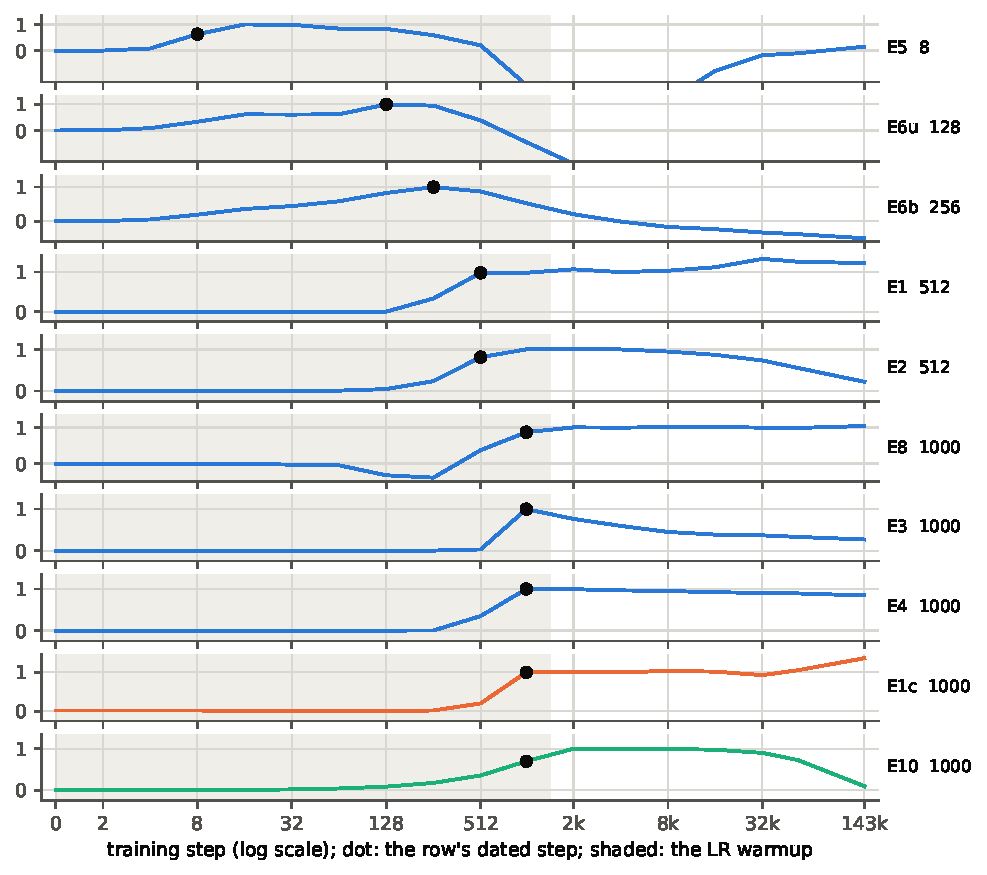
\includegraphics[width=\linewidth]{fig/fig2_timeline.pdf}
\caption{Seed 0's rows by step, each as the share of its change ($\Delta $ over its reference; E1 as V over its plateau median, E1c as $V_c$ at $10^{-4}$ over its own; the n-gram rows as the fall into their minimum), each signed so that its dated change is upward (E5, E2 and E8 fall). The axes are cut at $-$1.2, and E5 and E6u run below the cut after their dates. Dot: the dated step (E8's dated from step 0, 1000; from its peak it is 512). Shaded: the warmup, to step 1430. E7 and E11 are not drawn. Each panel is shown and read on its own in appendix~\ref{sec:D}.}\label{fig:fig2_timeline}
\end{figure}

\textbf{The order.} E5 (8) < E6u (128) < E6b (256) < E1 = E2 (512) < E3 = E4 = E1c = E10 (1000), with E8 between the two groups: dated from step 0 it ties the second (1000), dated from its peak the first (512). The rank collapse and the unigram minimum come before the break; the break falls with the OV fall, within one grid step of the bigram minimum and of the previous-token and induction heads, which the centred cloud's break joins (on the seeds too, at 1000 on eight of nine). E1c was added after the other rows were read and its pairs are not counted below. The 11 pairs fixed before the reading are the break with each of the nine model and simulator rows, and two among the circuit rows (E4 with E3, E3 with E2). Seven are aligned within one grid step, 2 are not (the rank collapse and the unigram minimum come first) and 2 are unread (E7 censored, E11 refused). A one-step gap counts as aligned, here and in \S\ref{sec:1}. No null says how many pairs quantities driven by one ramp would align on this grid, so the count is description. For scale: most rows fall on the four consecutive grid steps 256, 512, 1000 and 2000, and two dates drawn independently and uniformly from those four are within one grid step with probability 10/16 = 0.625, and seven of the nine pairs read include the break, which sits at 512 between 256 and 1000, so that a date drawn the same way is within one grid step of it with probability 3/4. Seven aligned of nine read is about what chance placement on these steps gives; the alignments are not evidence of a link.

Two rows reverse after their dates, beside the break. The token cloud's effective rank (E5), which falls by step 8, climbs back past its starting value between 512 and 1000, the step at which the centred cloud breaks; induction attention (E3) peaks at 1000 and falls after. Neither second move is dated.

\textbf{Every aligned pair is inside the warmup.} The schedule's own row reads 1000 by construction (the learning rate reaches half its peak at step 715, between grid steps), and inside a linear ramp ``within one grid step'' includes ``driven by the same ramp''. Nothing in this table separates a training event from the schedule (\S\ref{sec:7}).

\textbf{``Break, then induction, then the OV phase'' is not shown.} The OV phase is named for E2, an eigenvalue share, so ``repulsive'' names that share's fall, not a negative feedback shown in the dynamics (\S\ref{sec:6}). In one reading the OV phase is E2's fall, and it starts with the break, at 512; in the other it is E2's bottom, its first step at its minimum, which is 1000, the step induction is dated. Either way the OV phase and the break or induction are tied on this grid, not ordered.

\textbf{Inside the 1000 tie} (description, read after the dates). The share of each change done at 512, the grid step before, orders the rows the half-point ties: the break 0.98, the OV fall 0.81, previous-token 0.35, induction 0.03; the schedule is 0.36 done, beside previous-token, and the centred cloud (E1c) is 0.19--0.24 done across its four tolerances, between induction and previous-token. On the seeds, with each run's own previous-token and induction heads picked by their scores at the last step, the two tie at 1000 on 8 of the 8 seeds where both are located; previous-token is further along at 512 on 7 (shares 0.40--0.48 against 0.007--0.085), seed 4 the other way, and on seed 3 the induction head is not located. Previous-token attention is further along than induction at 512, the order the stagewise literature reports (\S\ref{sec:2.2}); the grid cannot date the gap. The shares compare quantities of different kinds (a count, an attention weight, a learning rate), each against its own reference, so they order the rows only as description.

\section{Is the break the OV maps'?}\label{sec:6}

The monotonicity results of \S\ref{sec:2.1} need each head's value map tied to its symmetric scores, and the OV maps' attractive share falls at the break's step (\S\ref{sec:5}). So the first suspect is the OV maps turning away from symmetric, attracting maps. That share's fall is not by itself evidence of repulsion: a head's path back to the residual stream is low rank and nonsymmetric, and negative eigenvalues of one such map do not establish negative feedback \citep[Sec.~V\,B]{gao2026}. No edit below puts the model under those theorems' hypotheses (the QK maps, the MLPs and the layer norms are untouched), so neither outcome tests the theory; the edits ask whether the break needs the OV maps' asymmetry. On seed 0 we edited every head's OV map at once in the forward pass and counted V again, at step 0, 256 and the five steps 512, 1000, 2000, 4000 and 143 000; only the last five are labelled. Two edits ask whether the break is the OV maps' asymmetry: (a) each map replaced by its symmetric part; (b) each map's rotation removed, keeping its gain: restricted to the head's write space, the map's real Schur form W = U S $U^{\top}$ (U orthogonal, S block upper-triangular) has each 2 $\times $ 2 diagonal block of S replaced by its symmetric part, so the rotation is removed plane by plane in an orthonormal basis even when the map is not normal. Each edit is read against 40 random edits matched to it twice: each control's change has the edit's norm, and each control's map has the edited map's norm, head by head. A cell is \emph{lower} or \emph{higher} only beyond all 40, and only beyond what the edit's change of gain alone does (the map rescaled to the edited norm, read beside and not drawn). The MLP blocks, which add to the stream in parallel with attention, are never edited. In-context copying is read beside it, as the repeat gain G of a probe of 16 sequences of 96 random tokens repeated once (the mean loss on the first copy's positions minus that on the second's), at the four steps from 1000, where copying exists.

\begin{figure}[tbp]
\centering
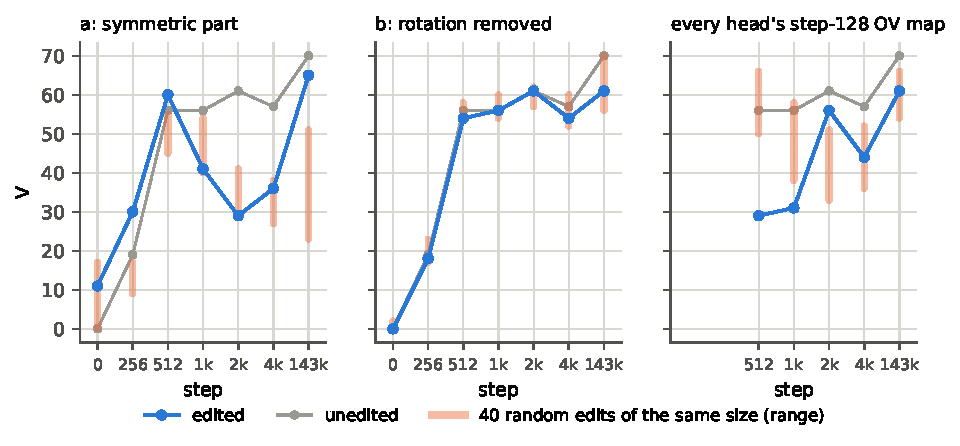
\includegraphics[width=\linewidth]{fig/fig3_ov.pdf}
\caption{V on seed 0 under each edit (blue) at the steps read, the unedited model (grey) and the range of the 40 matched random edits (orange). Left, (a) each OV map's symmetric part; middle, (b) its rotation removed; right, every head given its own step-128 OV map, against random edits matched to that substitution as above. The steps are evenly spaced; the gain-only control is not drawn, though a cell's label also requires the edit to go beyond it (\S\ref{sec:6}).}\label{fig:fig3_ov}
\end{figure}

\textbf{Neither edit undoes the break} (figure~\ref{fig:fig3_ov}). Under (a) V is lower than its controls at none of the five labelled steps and higher at 512 and 143 000; under (b) it is as its controls at every step. The controls show what (a) is: a large edit, random edits of its size alone moving V far from the unedited count and breaking most copying. Beside the labelled steps, (a) gives V = 11 at step 0, inside its controls' 0--17 (so a random edit of its size makes the initialised model non-monotone too), and 30 at 256, above all 40 (9--17). (b) is a small edit: removing the rotation changes a head's map by a median 0.08--0.10 of its norm. Copying survives it: G is 8.19--12.41 at the four steps, as its controls and about the unedited model's, where zeroing the OV maps of ten induction heads takes it to 1.06--2.57 (appendix~\ref{sec:B}).

\textbf{The one OV-only edit with a known destination does not reach it either.} Giving every head its own step-128 OV map, where V was 0, leaves V at 29--61 across the five steps. The edit is not inert: V is lower than every control at 512 (29 against 50--66) and at 1000 (31 against 38--58), and higher at 2000 (56 against 33--51), one grid step after the OV maps' attractive share reaches its lowest (\S\ref{sec:5}). The whole model moved to its step-128 weights, by contrast, gives V = 0 at every step from 512 to 4000. That is close to a tautology, since the step-128 model has V = 0 (\S\ref{sec:4}); it is a check that the count can register a reversal when one is made, not evidence about the OV maps. An OV-only edit does not take V there.

So the break is neither shown to be the OV maps' nor shown not to be. One OV-only edit with a known destination was tried, and it moves V in both directions without approaching monotone; the two structural edits show no reversal beyond random edits of their size. No other component (the MLPs, the layer norms, the embeddings, QK) was moved to its step-128 weights, so none of this is causal evidence about which components push the tokens apart.

\section{What would separate the schedule from training}\label{sec:7}

Every dated row of \S\ref{sec:5} from step 128 to 1000 falls inside the warmup, and the ten runs of \S\ref{sec:4} share it, so a break set by the ramp would reproduce exactly as this one does. Three kinds of run could separate the two: a model trained on the same schedule at a different peak rate; a suite with a different warmup and checkpoints inside it; and continued training from a checkpoint before the break, with and without the ramp. We ran the first two and read both dates, $E_{1}$'s break and the centred cloud's, by rules fixed before their outputs. A run of the second kind on Pythia itself exists and was found only after these were read: \citet{belrose2024} retrained \texttt{pythia-14m} and \texttt{pythia-70m} with a warmup of 14 300 steps, ten times Pythia's, to isolate its effect, and the checkpoints are released on Pythia's grid. Read from their figure, on 70m the minima of the KL divergence from a unigram and from a bigram predictor to the model (the divergence of rows E6u and E6b, \S\ref{sec:5}, but read on sequences sampled from the predictor, not on real text) come one to two octaves later under the longer warmup, so on that model those two rows move with the schedule. Neither of our counts has been read on that run.

\textbf{The predictions.} Each schedule says where a date at 410m's step should fall on another run: under \emph{step}, at the same count of updates; under the \emph{cumulative} learning rate (the dose the weights have received), where that run's summed rate reaches 410m's at the date; under the \emph{instantaneous} rate, where its rate does. Each is mapped from 410m's dates on the ten seeds (256--512 for the break, 512--1000 for the centred date) onto the other run's grid as a band. A date g on the grid stands for a crossing somewhere in (g$'$, g], g$'$ the grid step before it; inside a linear warmup each schedule carries a step t on 410m to f$\cdot $t on the other run (f = 1 for step, $\surd $(p/p$'$) for the cumulative rate and p/p$'$ for the instantaneous one, p and p$'$ the two peak rates; on GPT-2 small, whose warmup is logarithmic, its rate at step n is taken as p$'$ ln n / ln W$'$, W$'$ its warmup's length, the form its logged rate follows, and the cumulative map inverts that rate's integral), and the band is every grid step s of the other run whose own interval (s$'$, s] meets (f$\cdot $g$'$, f$\cdot $g] for some date g in 410m's range. A run's dates keep the schedules whose bands contain them. The schedules are deterministic functions of the step, so a date consistent with one is not evidence that it causes anything.

\begin{figure}[tbp]
\centering
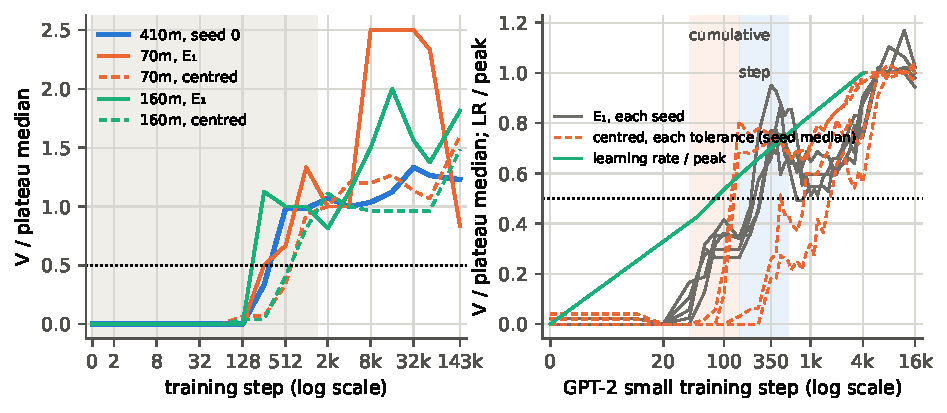
\includegraphics[width=\linewidth]{fig/fig4_schedules.pdf}
\caption{Left, V over its plateau median on \texttt{pythia-70m} and \texttt{pythia-160m} ($E_{1}$ solid, the centred cloud at $10^{-4}$ dashed) and on seed 0 of \texttt{pythia-410m}, with the half line; 70m's $E_{1}$ is over a plateau of only 6 drops, which is why its curve reaches far above 1. Right, on Mistral GPT-2 small's five seeds (grey, not told apart), V over each seed's plateau median as the rule fixed before that run took it, with the half line; dashed, the centred count at each of its four tolerances, over its own plateau, the median over the seeds (they disagree, which is why no centred date is read); green, the logged learning rate over its peak (logged to step 4100); shaded, the bands where the cumulative rate (left) and the count of updates (right) put $E_{1}$'s break. Shaded on the left: Pythia's warmup. Step 0 is drawn where step 1 would be.}\label{fig:fig4_schedules}
\end{figure}

\textbf{Pythia 70m and 160m.} They have 6 and 12 layers (so V is at most 6 $\times $ 7 and 12 $\times $ 7, against 24 $\times $ 7 for 410m), and they warm up over the same 1430 steps at peak rates of $10^{-3}$ and 6 $\times 10^{-4}$, against 3 $\times 10^{-4}$ for 410m, so the cumulative and instantaneous rates reach 410m's earlier in steps. On both, $E_{1}$'s break is at 256 and the centred date at 1000, the same at every tolerance (figure~\ref{fig:fig4_schedules}). Under the instantaneous rate the centred date is predicted at 256--512 on 160m and 128--512 on 70m, so the rate itself is excluded; on 160m step predicts 512--1000 and the cumulative rate 256--1000, both containing 1000. $E_{1}$'s break at 256 excludes none of the three: all their bands contain it. The joint reading is \textbf{consistent with step and cumulative}, and it is the same without 70m's $E_{1}$ date, which rests on a plateau of 6 drops, so a few drops move it. Step against the cumulative dose is not told apart on Pythia's grid; size changes with the rate, and there is one seed per size (PolyPythias also releases seeds of 70m and 160m, not read here).

\textbf{Mistral GPT-2 small.} Stanford CRFM's Mistral trained five seeds of a GPT-2 small, each with its own random seed \citep{karamcheti2021}; we read the released checkpoints, every 10 steps to 100, every 50 to 2000 and more sparsely after \citep{crfm}, and take its states as for Pythia (the embeddings, each block's output, the last after the final layer norm). Its learning rate rises logarithmically, reaching half its peak of 6 $\times 10^{-4}$ by step 100 and the peak at about step 4000, as logged in each seed's released trainer state, so the cumulative dose predicts far earlier dates than step does, and here the schedules separate: for $E_{1}$'s break the cumulative band is 40--150, step's 150--550. $E_{1}$'s break falls at 250 or 350 on all five seeds, in step's band only, and the frozen joint reading is \textbf{``consistent with step''}. The rule fixed before the run said this label would narrow the claim that nothing separates the schedule from training. We decided after reading the run, and before writing this section, not to let it, for three reasons:

\begin{itemize}
  \item \emph{$E_{1}$ rises in two stages} on every seed (figure~\ref{fig:fig4_schedules}): to 14--17 drops by step 100, inside the cumulative band, then to 31--39 by 350, inside step's. The frozen plateau (the median over 4000--16 000: 410m's window carried by tokens seen, since a GPT-2 small step sees a quarter of a Pythia step's tokens) puts its half between the stages; against 410m's own window, 1000--4000, the half-rise reads 80 or 200, and the joint would read ``neither''. The label holds for the larger stage and depends on the window.
  \item \emph{The centred count gives no date.} Each seed's four tolerances disagree, from 100--2000: the two fixed tolerances jump at 100--150, in the cumulative band, the two derived ones rise slowly and date 350--2000. By the rule a disagreement widens a seed's date to its span, and step survives the centred count on four seeds only through the tolerance matched to the re-initialised models, which is set by their single largest drop; at the next value the joint reads ``neither''.
  \item \emph{Neither schedule maps the whole curve.} Under step, 410m has nothing at GPT-2's first stage (V is 0 through 128); under the cumulative dose, GPT-2's first stage maps onto most of 410m's rise, where GPT-2 is still far below its plateau.
\end{itemize}

So on another suite with a different warmup, the break's larger rise falls where the count of updates predicts, after a first rise where the dose does, and the centred cloud's single date of \S\ref{sec:4.1} does not transfer. Nothing here separates a training event from the learning-rate schedule on \texttt{pythia-410m}. For \texttt{pythia-70m} the long-warmup run could: it differs from the \texttt{pythia-70m} read above in its warmup (its other settings are not published with it), and on its grid the instantaneous rate puts both dates far from where the count of updates does, while the cumulative rate's band is apart from step's only if 70m's own dates are known to within a grid step (one seed read so far). For \texttt{pythia-410m} it is the third kind: continued training from a checkpoint before the break with the ramp replaced by a flat rate, on a model whose circuit is known.

\section{Related work}\label{sec:8}

\textbf{Geometry along the training axis.} Several works read a global geometric statistic of hidden states along Pythia's checkpoints. \citet{li2025} find three phases in the spectrum of the last layer's representations (RankMe, $\alpha $ReQ), the first coinciding with the learning-rate ramp. \citet{billa2026} finds task representations' RankMe collapsing from step 0 to steps 32--256 on Pythia 160m and 410m and partly recovering by about step 1000. \citet{cheng2024} follow intrinsic dimension by layer from step 512, and \citet{razzhigaev2023} report intrinsic dimension rising and then falling over training. A non-monotone geometric arc along training is therefore not new, and neither is the statistic in kind: at $\beta $ = 1, $E_{1}$'s first-order term is $\tfrac12\|m\|^{2}$, half the anisotropy measure $\|m\|^{2}$ (\S\ref{sec:2.1}). What is new here is reading the particle picture's prediction, $E_\beta $ monotone in depth, along a real training axis, on checkpoints inside the first 1000 steps: the step at which it breaks, that step's reproduction across seeds, and its place on the developmental order. The nearest published reading along Pythia's checkpoints, of the representations' entropy and the first token's norm, reads no step between 1 and 1000 \citep{queipo2025}.

\textbf{Anisotropy, outlier dimensions and sinks.} $E_\beta $ is a moment of the tokens' Gram matrix, so it moves with anisotropy, the tokens' shared direction. Contextual representations are anisotropic in every layer but the input \citep{ethayarajh2019}, and anisotropy appears in Transformers trained with other objectives and on other modalities \citep{godey2024}; a few rogue dimensions dominate similarity measures between them \citep{timkey2021}; trained transformers' representations are dominated by one principal direction \citep{benartzy2026}, and decoders' anisotropy, the top principal direction's share of the centred representations' variance, peaks in their middle layers \citep{razzhigaev2023}. That measure removes the mean, so it is not $\|m\|^{2}$: \S\ref{sec:4.1}'s profile of $\|m\|^{2}$ rises with depth before the break and falls at several transitions after it, but whether a peak of their kind forms at the break would be read on the centred cloud, and was not. Large language models carry a few activations of very large magnitude that act as fixed biases \citep{sun2024}, and attention concentrates on initial tokens that act as sinks \citep{xiao2023}. At the break's steps the massive coordinates do not carry the mean \S\ref{sec:4.1} removes or its falls: they are ordinary there and reach their size only from step 16 000 (\S\ref{sec:4.1}); the sinks are not examined. Along Pythia's training, \citet{queipo2025}, who prove that a token of massive norm forces the representations into compression, read the matrix entropy, the attention-sink rate and the first token's norm of \texttt{pythia-410m} and larger models at steps 1, 1000, 2000, 4000 and later, on one prompt, and find all three ``emerge together around step 1k''. Their statistics are close kin to ours (the matrix entropy, and the anisotropy they read in depth, the top singular value's share of the representations' squared norm, are spectral readings of the uncentred representations, as $\|m\|^{2}$ is), and theirs is the nearest published reading to this paper's; but their first read after step 1 is step 1000, so their date places those changes in (1, 1000], which contains both of our dates and does not order them. Their criterion for massive activations (the first token's norm) is not ours (one coordinate's largest value against the median coordinate's), and our coordinates reach 100$\times $ only at 16 000--32 000, so the two dates are not one quantity. \citet{bernas2026} study anisotropy chiefly through the gradients, with activations read from step 10 000 on. \S\ref{sec:4.1} reports the energy on token-centred clouds, the control this calls for. Pure attention loses rank with depth \citep{dong2021}, and rank collapse at initialisation hinders training \citep{noci2022}; our row E5 reads the token cloud's rank along training.

\textbf{Warmup.} The warmup is commonly explained as controlling the adaptive optimiser's early variance \citep{liu2019} or as moving the model to regions that tolerate larger learning rates \citep{kalra2024}. Both make the schedule a plausible cause of any event inside it, which is why \S\ref{sec:7} does not separate the two. The confound is not new: \citet{olsson2022} note that their small models' phase change overlaps the warmup, \citet{chen2023} re-plot their transition against the weights' distance from initialisation and the optimisation path's length, and PolyPythias' representational shift peaks near the end of the warmup \citep{vanderwal2025}.

\textbf{Developmental interpretability.} The stagewise picture of \S\ref{sec:2.2} comes from the local learning coefficient \citep{hoogland2024}, refined per head \citep{wang2024}, and from susceptibilities \citep{wang2025}; induction heads \citep{olsson2022} and the function-vector heads many of them become \citep{yin2025} are its best-studied circuit, and how an induction head forms has been studied mechanistically \citep{singh2024}. Abrupt structure formation during training, with a sudden drop in the loss, is reported in masked language models \citep{chen2023}. PolyPythias \citep{vanderwal2025} reports training dynamics highly consistent across seeds, with outlier runs; \S\ref{sec:4}'s seeds include two such runs.

\textbf{Theory.} The particle picture of self-attention, its clustering and metastability, are developed in \citet{geshkovski2023,geshkovski2024}, \citet{bruno2024} and \citet{rigollet2025}; the monotonicity conditions of \S\ref{sec:2.1} are in \citet{geshkovski2023} and \citet{pendharkar2026}. \citet{gao2026} study the repulsive case (Q = K = I, V = $-$I) as a recurrent discrete map with normalisation and find that it need not settle: on the circle the regular polygon loses stability to period-two motion, chaos and flipping clusters, and attention can condense onto a few partners without the tokens clustering. \citet{isobe2026} train a noisy mean-field model's feed-forward part and find tokens leaving the clustered regime near the final layers, already after one gradient step, a predicted shape with no checkpoints; our drops instead sit in the middle of the stack at the break and are absent through step 128 (appendix~\ref{sec:C}). \citet{koubbi2026} let the weights vary randomly across layers and heads, as at initialisation, and derive the overlaps' dynamics in depth (\S\ref{sec:2.1}). \citet{herty2026} couple the tokens' flow in depth with the parameters' flow in training, as theory.

\textbf{Earlier notes.} The author's informal notes compared trained GPT-2, ALBERT and BERT models with random weights of matched norm: under random weights the energy rose monotonically in depth, as the identity-weight picture predicts, and in every trained model, prompt and $\beta $ tested it did not. They read only endpoints; \S\ref{sec:4} dates when, along training, the monotonicity is lost.

\appendix

\section{The shared subspaces}\label{sec:A}

Do the 384 heads come to query, key, read and write the same directions of the residual stream, and when? This appendix is context for \S\ref{sec:6}, read along the same steps, and no claim above rests on it; whether its OV readings predict the step-128 substitution's effect is not read. For each family of per-head subspaces (query, key, OV write, OV read, and the OV map's invariant subspaces with negative real, positive real and complex eigenvalues) we average the heads' orthogonal projectors and take the participation ratio PR of the mean. Under a null that rotates each head's subspace by an independent Haar rotation PR has an exact expected value $\operatorname{PR}_{0}$, and $\rho $ = PR / $\operatorname{PR}_{0}$ is 1 under it and falls as the heads concentrate on shared directions. Each step's PR is read against the null's range over its draws. The Haar null, a Gaussian draw of the weights matched in norm, and the step-0 weights give the same distribution of PR, and every step is read against it. $\rho $ is a description: a count of shared directions cannot be calibrated on a trained pool, and neither can $\rho $'s effect side, because a planted shared direction added to the pool lowers $\rho $ mostly by diluting the pool's own concentration, so a planted effect's size says nothing about a real one. The readings use the weights only, except the comparison with the residual stream's top-variance directions below, which uses the seven prompts. Figure~\ref{fig:fig11_rho} draws $\rho $ by family and step.

Through step 128 every family reads the null (|$\rho -$ 1| at most 9.4 $\times 10^{-4}$ in the OV families and 4.5 $\times 10^{-4}$ in QK). The query and key families leave it at 256, with the OV write (256) and OV complex (256) families; OV read, negative and positive follow at 512. All of this is inside the warmup, at or before the break. OV write is the most concentrated family at 512 and 1000 ($\rho $ 0.89 and 0.66); from 2000 the query family is ($\rho $ 0.50), and from 4000 the query and key families both are, ending at 0.51--0.53 against the OV families' 0.65--0.82 at the last step. The shared spaces are not the residual stream's top-variance directions at any step, and at the last step the OV write, negative and complex ones partly coincide with 410m's massive-activation coordinates, which they avoid through 4000.

\begin{figure}[tbp]
\centering
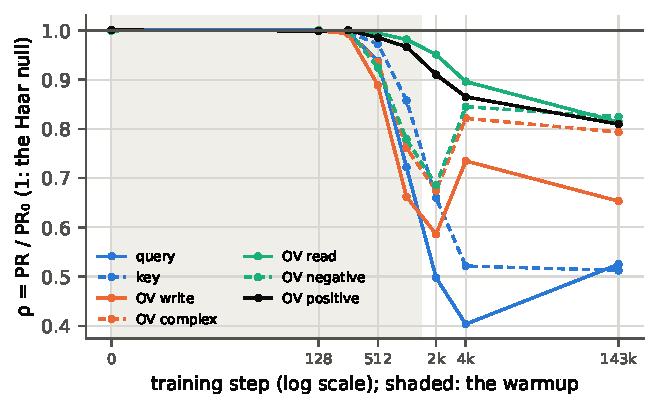
\includegraphics[width=0.75\linewidth]{fig/fig11_rho.pdf}
\caption{$\rho $ = PR / $\operatorname{PR}_{0}$ for each family of the 384 heads' subspaces at the eight steps read, on seed 0 (1 under the Haar null; lower, the heads share directions). Through step 128 every family is within $10^{-3}$ of 1. Shaded: the warmup, to step 1430.}\label{fig:fig11_rho}
\end{figure}

\citet{shaikh2026} read an overlap of heads' projections in the weights of four larger models, with checkpoints on OLMo-2 only: keys grow most, queries the same way more gently, values stay near-orthogonal throughout. Our key family agrees in direction. Their value statistic is not our OV read family (a different subspace, pooled differently), so the two are not compared.

\section{The gates, and why each null is the one used}\label{sec:B}

Each reading above was gated before it was read: the full statistic was run on inputs whose answer is known, on a planted null and on a planted effect at the real design points, and the real data were read only once every arm passed. Where an arm failed, the failure and the change are stated where the reading is.

\textbf{The break's half-rise (\S\ref{sec:3.3}, \S\ref{sec:4}; the gate of \texttt{P-A5} on seed 0).} \emph{Known answer:} seed 0's energies reproduce an earlier CPU run to a relative 1.5 $\times 10^{-6}$ (the gate's tolerance $10^{-4}$), and V exactly. \emph{Planted breaks:} a synthetic series breaking at each grid step is read at that step for 2, 4, 8, 16, 32, 64, 128, 256, 512, 1000, 2000; one planted at 4000, the plateau's last step, reads 2000, since the plateau then contains the rise; a series is read inside the window exactly when its break was planted there. \emph{Planted null:} 20 000 draws of the nine seeds' steps from the uniform-location null, through the scorer, reproduce Bin(9, 1/6) for K (largest standardised gap 2.4); this checks the scorer, and the planted breaks check the half-rise rule. \emph{Planted effect:} seed 0's series moved one grid step later reads 1000, outside the window. \emph{Sensitivity:} the date is the same at every tolerance and with any one prompt left out (\S\ref{sec:3.2}). \emph{Why this null:} it is the alternative to ``the recipe sets the step'', scattering each run's step over the early grid. Nobody holds it, which is why beating it is cheap (\S\ref{sec:4}).

\textbf{The locator (\S\ref{sec:5}).} Each row's no-change null (bootstrap draws of the row with its change removed) reads ``no change'' in at least 0.972 of 1000 draws, and changes planted in each gap of the grid at the row's own noise are placed in the right gap. The first gate failed on four rows whose spread grows by orders of magnitude over training; the revised gate, with each row's floor on its own spread, passes on every row dated, and the simulator's row (E11) is refused. \emph{Why:} a date is only as good as the locator's power to tell a change from none in each gap.

\textbf{The OV edits (\S\ref{sec:6}).} Random edits are never labelled lower or higher against their own controls (0 labels). Zeroing ten induction heads' OV maps loses copying at four of four steps (G 1.06--2.57). Moving the whole model to its step-128 weights lowers V below its controls at four steps at full dose, to V = 0, so the count can see a reversal when one is made. A displacement guard, meant to leave unread any cell whose edit moves the residual stream further than its controls, refused both planted effects, and was made description before any arm was read; it is not reported here. \emph{Why random edits matched in size and in each head's norm:} a structured edit has to be told from what any edit of its size does, and the gain change alone is read beside, because the scale of a head's map moves V by itself.

\textbf{The centred counts (\S\ref{sec:4.1}, \S\ref{sec:7}).} The steps no schedule reaches (0--128 on Pythia, 0 and 10 on GPT-2 small) are read first, and a centred count there of half its plateau or more would refuse the control; none did. The two derived tolerances are fixed per model before its records: one so that the re-initialised models' centred drop rate matches their uncentred one (the same architecture with fresh random weights; on GPT-2 small this tolerance is set by a single largest drop of theirs), one so that a planted spread is seen by the centred count as by the uncentred one; each tolerance is gated on the re-initialised models and on two planted effects (a common vector added to every token, which the centred count must not see, and a spread, which it must). The common vector is added to each token's residual state before it is normalised to the sphere, scaled by the median token norm, so centring the unit cloud does not remove it exactly; the gate asks that the centred count not see it all the same. One tolerance on the centred energy's own scale, meant to compare the two counts' sizes, failed its own gate, which is why only dates are compared. The centred rules were frozen after a preflight, which runs the statistic on step 0, a matched random initialisation, the trained population at a step off the scored grid, and a planted control at dose 0 and three doses; its refusals are fixed or argued in the design.

\section{What the count is made of}\label{sec:C}

Read from the same records as \S\ref{sec:4} and \S\ref{sec:4.1} after every date there was read (description; no rule, no threshold; the readings were fixed before their output, and none replaces a date above).

\begin{figure}[tbp]
\centering
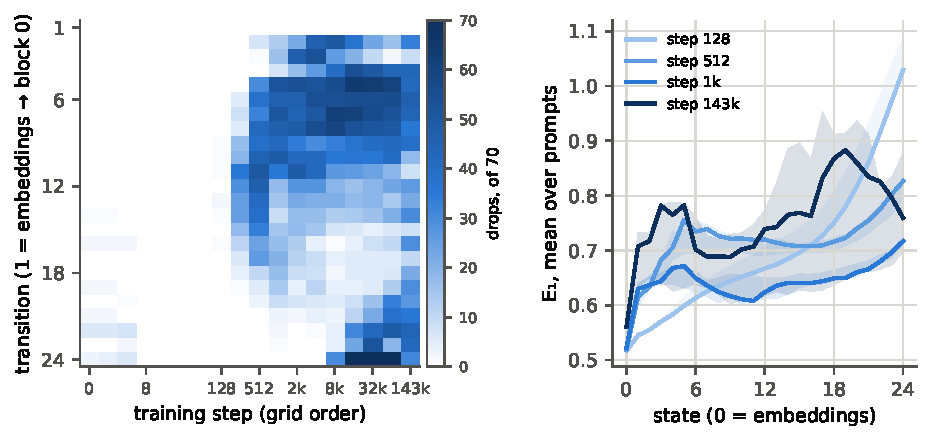
\includegraphics[width=\linewidth]{fig/fig5_count.pdf}
\caption{Left, the drops at each of the 24 transitions (rows, 1 = embeddings into the first block, 24 = into the final layer norm) and each step (columns), summed over the 7 prompts and the ten seeds (at most 70 per cell). Right, $E_{1}$ by state, averaged over the prompts, at four steps: seed 0 as a line, the other nine seeds' range as a band.}\label{fig:fig5_count}
\end{figure}

\textbf{By prompt.} Each prompt's own count, dated by the same half-rise on its own 1000--4000 level, breaks inside (128, 512] on 65 of the 70 prompt-and-seed series; the other five are one prompt, the Camus passage, the only one not in English, at 1000, each on a different seed. At each seed's break the largest share of V one prompt holds is 0.17--0.24.

\textbf{By layer.} At 256 and 512 the drops sit in the middle of the stack: the median drop is at transition 12 and 11, and most fall at transitions 10, 11 and 12 at 512. At 1000 they spread shallower (median 9; most at 5, 7 and 10).

\textbf{Without the frame-changing transitions.} The first and last transitions hold none of the drops at 256, 512 and 1000 and a share 0.05 of them at 143 000. V counted over transitions 2 to 23 alone dates every seed's break at the same step as V does (256 or 512), all ten inside the window.

\textbf{Net change.} On all 70 prompt-and-seed series at every step, $E_{1}$ after the last state is above $E_{1}$ at the embeddings; the median rise is 1.02 of the starting value at 128, 0.54 at 512, 0.36 at 1000 and 0.41 at 143 000. From state 1 to state 23 (leaving out both frame-changing transitions), the rise holds on 39--63 of the 70 from step 8000 on and on all 70 before. So a drop is a dip inside a net rise, not a fall of the whole profile.

\textbf{A later plateau.} With the plateau taken at 8000, 16 000 and 32 000 the dates are 256 and 512; only seed 9 moves, from 256 to 512.

\textbf{Which coordinates carry the mean.} Figure~\ref{fig:fig9_massive} draws \S\ref{sec:4.1}'s massive-activation reading by step: the massive-activation coordinates' largest value on all ten seeds (figure~\ref{fig:fig10_level} draws the level).

\begin{figure}[tbp]
\centering
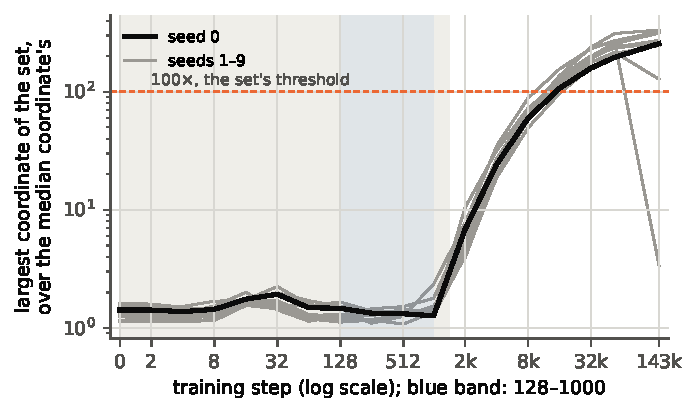
\includegraphics[width=\linewidth]{fig/fig9_massive.pdf}
\caption{For each seed, the largest of its massive-activation coordinates (one set per seed, fixed over the whole grid) over the median coordinate's, by step; seed 0 in black. Blue band: steps 128--1000, where both of \S\ref{sec:4}'s events fall. Dashed: the 100$\times $ threshold that defines the set. On seeds 3 and 4 the curve falls at the last step, on seed 4 far below the threshold: their carriers change late, which is why the set is the union over the grid, not the set at the last step.}\label{fig:fig9_massive}
\end{figure}

\section{The timeline's rows, one by one}\label{sec:D}

This appendix takes table~\ref{tab:rows}'s rows one at a time, in the table's order, each with its own panel of figure~\ref{fig:fig2_timeline}. Every entry answers the same four questions: what the row measures, why it is on the timeline, how it is dated, and whether its change is larger than its noise. Table~\ref{tab:rowsD} puts the numbers side by side; a row's name links to its entry. Every row is on seed 0, at the 18 steps.

\textbf{Reading a panel.} The vertical axis is the share of the row's change done by each step: $\Delta $(s) over the row's reference (\S\ref{sec:5}), signed so that the dated change is upward. The solid line at 1 is the reference, and the hollow ring marks the step it is taken at; the dashed line at $\tfrac12$ is the half-point, and the dot is the dated step, the first grid step on or above it. E6u and E6b are dated at their minimum instead, so their panels have no half-line and the dot sits on the ring. The shading is the learning-rate warmup, to step 1430. A date means that half the change is done by that step and not by the grid step before it; nothing between grid steps is seen.

\textbf{What ``larger than its noise'' means.} For every row dated by the locator, $\sigma $ is the bootstrap standard error of $\Delta $ at the reference step, over 1000 resamples of the row's units (its prompts, heads, layers or text blocks). The row is dated only if the reference is at least 4$\sigma $; otherwise it reads ``no change''. Each row's own floor was also calibrated, as the 95\,\% upper bound of the 95th percentile of reference / $\sigma $ over 1000 flat series carrying that row's noise, and the floor used is the larger of the two; every row's own bound came out under 4. Before any row was dated, the rule was run on 1000 flat series per row, which read ``no change'' at least 95\,\% of the time, and on a change planted in each gap of the grid at 9$\sigma $, which it placed in the right gap at least 90\,\% of the time (appendix~\ref{sec:B}). Passing the floor says the row's early change is not noise across its own units. It is not a p-value for the date, and it does not test whether two rows' dates are linked, which \S\ref{sec:5} reads as description. With 7 prompts as units, $\sigma $ is the spread over these seven texts, not over text in general.

\begin{table}[htbp]
\centering\small
\caption{The rows' numbers. Reference: the row's largest change from step 0 up to step 4000, at the step given (for the n-gram rows, the fall into the minimum). $\sigma $: its bootstrap standard error over the units. Null: the share of 1000 flat series at the row's noise that read ``no change''. E1, E1c and E10 are not dated by the locator, so they have no $\sigma $; E11 has no date.}\label{tab:rowsD}
\begin{tabular}{@{}l l r r r r l@{}}
\toprule
row & units & reference (step) & $\sigma $ & ref / $\sigma $ & null & dated \\
\midrule
\hyperref[sec:D:E5]{E5} & 7 prompts & 12.53 (16) & 0.604 & 20.7 & 0.972 & 8 \\
\hyperref[sec:D:E6]{E6u} & 64 blocks & 1.84 (128) & 0.016 & 118.4 & 1.000 & 128 \\
\hyperref[sec:D:E6]{E6b} & 64 blocks & 3.60 (256) & 0.026 & 140.4 & 1.000 & 256 \\
\hyperref[sec:D:E1]{E1} & 7 prompts & --- & --- & --- & --- & 512 \\
\hyperref[sec:D:E2]{E2} & 384 heads & 0.504 (1000) & 0.002 & 226.7 & 1.000 & 512 \\
\hyperref[sec:D:E8]{E8} & 24 layers & 9.28 (2000) & 1.11 & 8.3 & 1.000 & 1000 \\
\hyperref[sec:D:E3]{E3} & 14 (prompt, head) & 0.060 (1000) & 0.005 & 11.9 & 0.990 & 1000 \\
\hyperref[sec:D:E4]{E4} & 7 prompts & 0.911 (1000) & 0.008 & 120.6 & 0.984 & 1000 \\
\hyperref[sec:D:E1c]{E1c} & 7 prompts & --- & --- & --- & --- & 1000 \\
\hyperref[sec:D:E10]{E10} & --- & --- & --- & --- & --- & 1000 \\
\hyperref[sec:D:E7]{E7} & 24 layers & 2.38 (4000) & 0.082 & 29.2 & 1.000 & censored at 2000 \\
\hyperref[sec:D:E11]{E11} & 7 prompts & --- & --- & --- & --- & refused \\
\bottomrule
\end{tabular}
\end{table}

\subsection{E5: the token cloud's effective rank}\label{sec:D:E5}

\begin{center}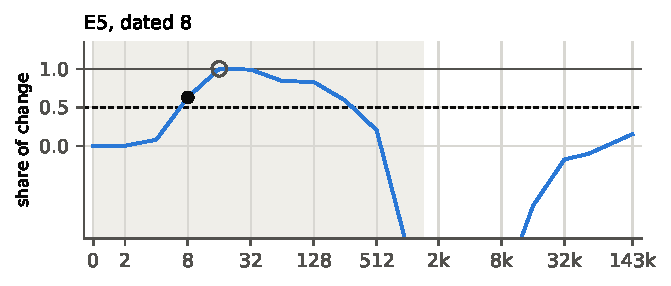
\includegraphics[width=0.7\linewidth]{fig/figD_E5.pdf}\end{center}

\textbf{What it measures.} For each prompt and state, the effective rank exp($-\sum _{k} p_{k} \ln p_{k}$) of the unit tokens' Gram matrix, $p_{k}$ its eigenvalues over their sum: roughly, how many directions the tokens spread over. The row takes the smallest value over the 25 states, so it reads the layer where the cloud is narrowest, and averages it over the 7 prompts. It falls when, at some layer, the tokens crowd into a few directions.

\textbf{Why it is on the timeline.} Rank collapse, tokens becoming nearly parallel with depth, is studied in the theory of attention \citep{dong2021,noci2022}, and in its simplest form it is the clustering the particle picture predicts. A row that dates it says whether the clouds narrowed before or after the energy broke.

\textbf{How it is dated.} It starts at 14.66 at step 0 and reaches 2.12 at step 16, its lowest value up to 4000, so the reference is a fall of 12.53; more than half of it is done by step 8.

\textbf{Larger than its noise?} Yes: the reference is 20.7$\sigma $ over the 7 prompts. Its null arm read ``no change'' on 0.972 of the flat series, the lowest of the rows and still above 0.95.

\textbf{What to take from it.} This is the table's earliest change, long before the break. It reverses: the rank climbs back past its starting value between 512 and 1000, the step at which the centred cloud breaks, and ends at 12.75. The panel cuts its fall below $-$1.2. Only the first move is dated.

\subsection{E6u and E6b: how close the model is to a unigram and a bigram predictor}\label{sec:D:E6}

\begin{center}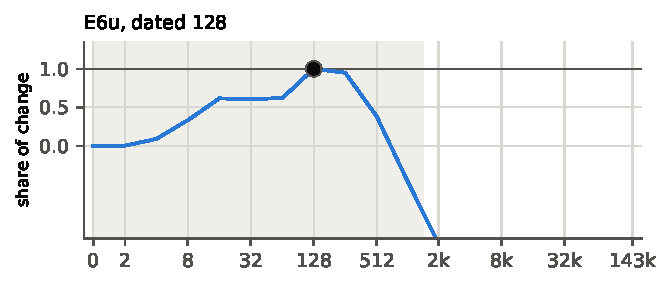
\includegraphics[width=0.7\linewidth]{fig/figD_E6u.pdf}\\[2pt]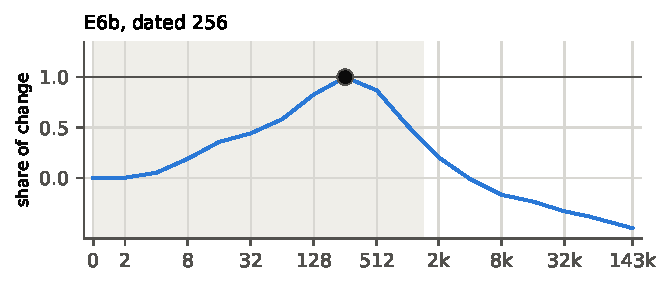
\includegraphics[width=0.7\linewidth]{fig/figD_E6b.pdf}\end{center}

\textbf{What they measure.} KL($q \,\|\, p_{\text{model}}$) in nats, from a predictor q to the model's next-token distribution. For E6u q is a unigram predictor (token frequencies), and for E6b a Witten--Bell bigram predictor, both counted on 2 000 000 held-out tokens of the Pile's validation split. The KL is averaged over the positions of a block of 1024 tokens and over 64 such blocks. A small value means the model predicts much as the n-gram predictor does.

\textbf{Why they are on the timeline.} Networks fit low-order statistics of their data first, and on Pythia the loss on sequences sampled from unigram and bigram statistics falls to a trough and then rises \citep{belrose2024}. These two rows date that stage on this model, with the same locator as the other rows. Their appendix also reads this KL divergence, in the same direction, on sequences sampled from the predictor; ours is on real text. On \texttt{pythia-70m} retrained with a ten times longer warmup, its minima come later (\S\ref{sec:7}).

\textbf{How they are dated.} Both fall and then rise, so each is dated at its minimum, and the floor applies to the fall into it. E6u falls from 3.30 to 1.46 nats at step 128, and E6b from 5.52 to 1.92 at step 256. The bigram counted on a larger table (the rest of the split) also has its minimum at 256.

\textbf{Larger than their noise?} Yes, by far: 118.4$\sigma $ and 140.4$\sigma $ over the 64 blocks.

\textbf{What to take from them.} The model is closest to a unigram predictor at step 128 and to a bigram predictor at 256, one grid step apart. Both come before the break or one grid step before it, and both then move steadily away (to 8.59 and 7.32 nats at the last step). The panels cut E6u's later rise below $-$1.2.

\subsection{E1: the energy break}\label{sec:D:E1}

\begin{center}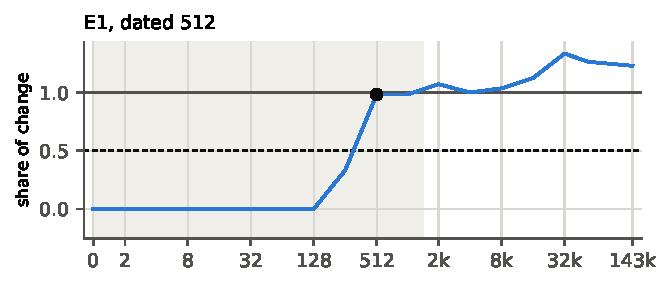
\includegraphics[width=0.7\linewidth]{fig/figD_E1.pdf}\end{center}

\textbf{What it measures.} V, the number of layer-to-layer drops in $E_{1}$ over the 7 prompts (\S\ref{sec:3.2}), here over its 1000--4000 plateau median (57).

\textbf{Why it is on the timeline.} It is the event the paper dates (\S\ref{sec:4}); the timeline asks what else changes when it does.

\textbf{How it is dated.} By the half-rise of \S\ref{sec:3.3}, not by the locator: V is 0 through step 128, 19 at 256 and 56 at 512, so it first reaches half the plateau at 512.

\textbf{Larger than its noise?} Its evidence is of a different kind. E1 is dated by the half-rise, not by the locator, so no $\sigma $ or floor is computed for it; instead its date holds at tolerances $10^{-4}$, $10^{-3}$ and $10^{-2}$ and with any one prompt left out (\S\ref{sec:3.2}), and it reproduced on 9 of 9 seeds under the prediction registered before their intermediate checkpoints were downloaded (\S\ref{sec:3.4}, \S\ref{sec:4}). It is the only registered row, and what the registration shows is that the date is the recipe's, not one run's.

\textbf{What to take from it.} The break is almost complete at 512 (0.98 of the change): of the rows dated 512 and 1000 it is the furthest along at 512.

\subsection{E2: the OV maps' attractive share}\label{sec:D:E2}

\begin{center}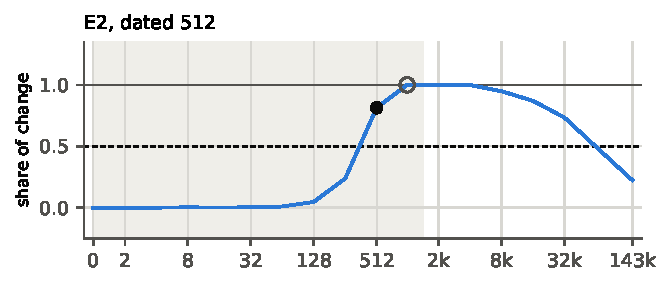
\includegraphics[width=0.7\linewidth]{fig/figD_E2.pdf}\end{center}

\textbf{What it measures.} For each head, the eigenvalues $\lambda $ of its OV map restricted to the head's 64-dimensional subspace, and the share $\sum _{\operatorname{Re}\lambda >0}|\lambda |^{2} / \sum |\lambda |^{2}$ of their squared size on eigenvalues with positive real part; the median over the 384 heads.

\textbf{Why it is on the timeline.} In the particle picture the value map decides whether tokens attract: with V = I they cluster and $E_\beta $ rises with depth, with V = $-$I it falls (\S\ref{sec:2.1}). A trained head's OV map plays V's part, and the share of its eigenvalues with positive real part is a head-by-head proxy for how attractive it is. If the break were the OV maps turning repulsive, this row would move with it.

\textbf{How it is dated.} It starts at 0.504, close to the half that a map with no preferred sign would give, and falls to 0.000 at step 1000: there the median head has no eigenvalue mass with positive real part. Half the fall is done by 512.

\textbf{Larger than its noise?} Yes: 226.7$\sigma $ over the 384 heads, the largest ratio in the table.

\textbf{What to take from it.} The fall is dated with the break, at 512, and its bottom at 1000 ties induction, which is why ``break, then induction, then the OV phase'' is not shown (\S\ref{sec:5}). A negative eigenvalue share is not by itself repulsion in the dynamics \citep{gao2026}, which is why the phase is named for the share; and editing the OV maps does not undo the break (\S\ref{sec:6}). The share recovers partway later, to 0.39 at the last step.

\subsection{E8: the weights' spectral tail exponent}\label{sec:D:E8}

\begin{center}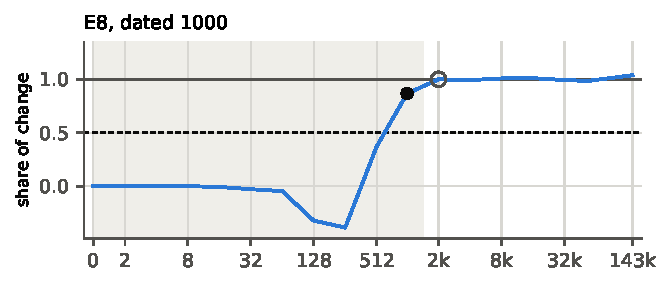
\includegraphics[width=0.7\linewidth]{fig/figD_E8.pdf}\end{center}

\textbf{What it measures.} For each weight matrix W, the exponent $\alpha $ of a power law fitted by maximum likelihood to the tail of the eigenvalues of $WW^{\top}$, the tail's lower cut chosen by the least Kolmogorov--Smirnov distance over tails of at least 10 eigenvalues; the median over the 24 layers, then over four matrix types (QKV, attention output, MLP in, MLP out).

\textbf{Why it is on the timeline.} In the heavy-tailed account of training, a smaller $\alpha $, a heavier tail, goes with more correlation learned into the weights \citep{martin2019}. With E2 and E7 it is read from the weights alone, with no input, so it says whether the weights' spectra change in the same window as the activations.

\textbf{How it is dated.} $\alpha $ first rises, from 13.52 at step 0 to a peak at step 256, then falls, to 4.23 at 2000. The locator dates only a move in the row's declared direction (down) from step 0, so the rise does not count: from step 0 the reference is 9.28 and the date 1000. Measured from the peak instead, the reference is 12.88 and the date 512. Both are given, and a pair with E8 is read only where the two agree (\S\ref{sec:5}).

\textbf{Larger than its noise?} Yes, but by the least margin of the dated rows: 8.3$\sigma $ over the 24 layers. That is under the 9$\sigma $ at which the first design called a row low-powered, though above the power calibrated for this row in its gap, which replaced that rule after the first gate and before E8 was dated (appendix~\ref{sec:B}).

\textbf{What to take from it.} The weights' tails grow heavy inside the window of the break and the circuit rows, and $\alpha $ stays near its new level to the end (3.88).

\subsection{E3: induction attention}\label{sec:D:E3}

\begin{center}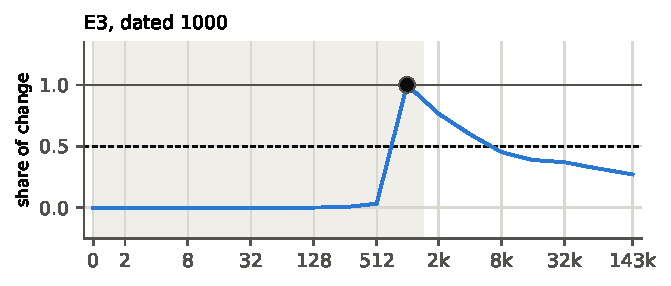
\includegraphics[width=0.7\linewidth]{fig/figD_E3.pdf}\end{center}

\textbf{What it measures.} The attention of heads \texttt{L8H6} and \texttt{L11H14} from a query to the key that follows an earlier copy of the query's token, pooled over every such pair in a prompt, weighted by the pairs' count over the 7 prompts and averaged over the two heads.

\textbf{Why it is on the timeline.} Induction heads complete a repeated pattern by attending to what followed the token's last occurrence, and their formation is a landmark of the developmental order (\S\ref{sec:2.2}; \citealp{olsson2022}). The two heads were named as induction heads in earlier work on this model, not picked from these series. The row as first written (five heads, attention to the earlier copy itself) was refused before it was read, because it scored the wrong key, and replaced by this one, which was gated before it was dated.

\textbf{How it is dated.} It rises from 0.004 to a peak of 0.065 at step 1000, and half of that is not reached until then: at 512 it is only 0.03 of the way.

\textbf{Larger than its noise?} Yes: 11.9$\sigma $ over the 14 (prompt, head) pairs.

\textbf{What to take from it.} Induction arrives late and abruptly, between 512 and 1000, the step at which the centred cloud breaks. It then falls, to 0.021 at the last step; the fall is not dated.

\subsection{E4: previous-token attention}\label{sec:D:E4}

\begin{center}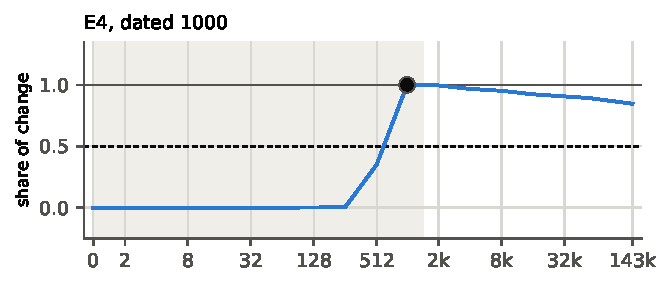
\includegraphics[width=0.7\linewidth]{fig/figD_E4.pdf}\end{center}

\textbf{What it measures.} Head \texttt{L5H2}'s mean attention from each query to the key just before it, mean over the 7 prompts.

\textbf{Why it is on the timeline.} Previous-token heads form before induction heads in the stagewise account (\S\ref{sec:2.2}), and an induction head reads from one \citep{olsson2022}. \texttt{L5H2} was named as this model's previous-token head in earlier work.

\textbf{How it is dated.} It rises from 0.014 to 0.925 at step 1000: by then the head puts nearly all its attention on the previous token. At 512 it is 0.35 of the way, so it crosses the half-point at 1000.

\textbf{Larger than its noise?} Yes: 120.6$\sigma $ over the 7 prompts.

\textbf{What to take from it.} Previous-token and induction tie at 1000 on this grid, but previous-token is further along at 512, the order the literature reports; the grid cannot date the gap (\S\ref{sec:5}). It stays high, at 0.78 at the last step.

\subsection{E1c: the centred cloud's break}\label{sec:D:E1c}

\begin{center}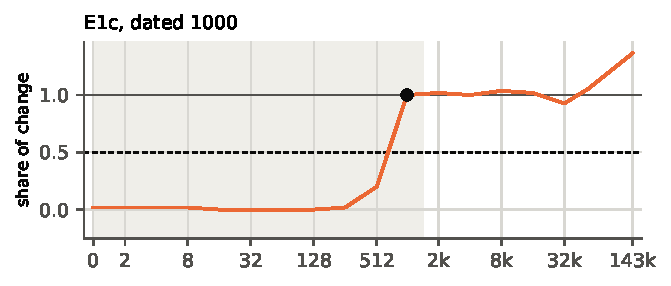
\includegraphics[width=0.7\linewidth]{fig/figD_E1c.pdf}\end{center}

\textbf{What it measures.} $V_c$, V counted on the token-centred cloud: each prompt's mean unit token removed and the rows normalised again (\S\ref{sec:4.1}). The panel is $V_c$ at tolerance $10^{-4}$ over its own plateau median.

\textbf{Why it is on the timeline.} $E_{1}$'s first-order term is the tokens' mean (\S\ref{sec:2.1}), so E1 can move with no change in how the tokens sit relative to one another. E1c dates the break with the mean removed. It was added after the other rows were read, so its pairs are not counted in \S\ref{sec:5}.

\textbf{How it is dated.} By the half-rise, at each of four tolerances; a date counts only if all four agree. At 512 it is 0.19--0.24 of its plateau, and all four reach half at 1000.

\textbf{Larger than its noise?} As for E1: dated by the half-rise, so no $\sigma $ or floor; its date holds at four tolerances and at 1000 on eight of the nine seeds, though it was not registered (\S\ref{sec:4.1}).

\textbf{What to take from it.} With the mean removed the break comes one grid step later, at the step of the circuit rows. The shared step is not read as a link: by \S\ref{sec:5}'s convention the uncentred break, one step earlier, is as close to them.

\subsection{E10: the learning-rate schedule}\label{sec:D:E10}

\begin{center}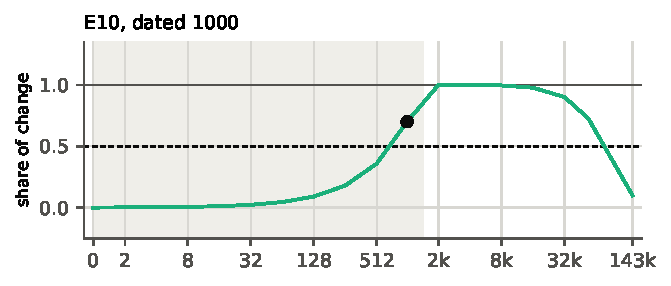
\includegraphics[width=0.7\linewidth]{fig/figD_E10.pdf}\end{center}

\textbf{What it measures.} Pythia's learning rate over its peak: linear to the peak at step 1430, then a cosine to 0.1 of it.

\textbf{Why it is on the timeline.} It is the confound. Every other row moves while the rate ramps up, so the schedule is dated with the same half-point to show where a row driven by the ramp alone would fall.

\textbf{How it is dated.} The rate reaches half its peak at step 715, between grid steps, so the first grid step past it is 1000. There is no noise and no floor.

\textbf{What to take from it.} Every aligned pair is inside the warmup, and nothing in the table separates a training event from the ramp (\S\ref{sec:7}).

\subsection{E7 and E11: the two rows not drawn}\label{sec:D:E7}\label{sec:D:E11}

\textbf{E7, the weights' relative change.} $\|W_{t} - W_{0}\|_{F} / \|W_{0}\|_{F}$ for each of the four matrix types, the median over the 24 layers, then over the types: how far training has moved the weights from where they started, a clock for training itself. It is 2.38 at step 4000, 29.2$\sigma $ over the 24 layers, and half of that is reached at 2000. But its largest change up to 4000 is at 4000 itself, still growing, so the reference is not the change's full size and the date is only a lower bound: censored. Its pairs are not read, and it is not drawn.

\textbf{E11, a simulator's cluster count.} The identity-weight dynamics of the particle picture, integrated from each step's measured token cloud to time 200 at a $\beta $ fitted to each prompt, and the number of clusters at the end (connected components of ``cosine $\geq $ 0.99''), mean over the 7 prompts. It asks whether the measured cloud, left to the idealised dynamics, would end in more than one cluster. It reads one cluster in every cell, as the theory requires at a long horizon \citep{geshkovski2023}, so it never changes and cannot date anything: refused. It is not drawn.

\bibliographystyle{plainnat}
\bibliography{refs}

\end{document}
